\documentclass[11pt,a4paper]{article}

% ---------------------------------------------------------------
% Paquetes
% ---------------------------------------------------------------
\usepackage[utf8]{inputenc}
\usepackage[T1]{fontenc}
\usepackage[spanish,es-tabla,es-nodecimaldot]{babel}
\usepackage{lmodern}
\usepackage[margin=2.5cm]{geometry}
\usepackage{booktabs}
\usepackage{tabularx}
\usepackage{longtable}
\usepackage{array}
\usepackage{amsmath}
\usepackage{amssymb}
\usepackage{pifont}
\usepackage{xcolor}
\usepackage{listings}
\usepackage{enumitem}
\usepackage{float}
\usepackage{graphicx}
\usepackage{etoolbox}
\usepackage{tikz}
\usetikzlibrary{arrows.meta,positioning,fit,backgrounds,calc}
\usepackage[hidelinks]{hyperref}
% Permite dividir URL y rutas largas en cualquier letra (equivalente a xurl)
\expandafter\def\expandafter\UrlBreaks\expandafter{\UrlBreaks
  \do\a\do\b\do\c\do\d\do\e\do\f\do\g\do\h\do\i\do\j\do\k\do\l\do\m\do\n\do\o\do\p\do\q\do\r
  \do\s\do\t\do\u\do\v\do\w\do\x\do\y\do\z\do\A\do\B\do\C\do\D\do\E\do\F\do\G\do\H\do\I\do\J
  \do\K\do\L\do\M\do\N\do\O\do\P\do\Q\do\R\do\S\do\T\do\U\do\V\do\W\do\X\do\Y\do\Z\do\_\do\-}

\definecolor{codebg}{RGB}{246,248,250}
\definecolor{codekw}{RGB}{0,92,197}
\definecolor{codecm}{RGB}{106,115,125}
\definecolor{codestr}{RGB}{3,47,98}
\definecolor{ok}{RGB}{26,127,55}
\definecolor{warn}{RGB}{154,103,0}
\definecolor{bad}{RGB}{176,30,30}
\definecolor{muted}{RGB}{90,96,104}
% Colores de los diagramas
\definecolor{dgline}{RGB}{60,66,74}
\definecolor{dggit}{RGB}{232,240,252}
\definecolor{dgjen}{RGB}{253,240,226}
\definecolor{dgdoc}{RGB}{228,244,236}
\definecolor{dgapp}{RGB}{243,236,250}

\lstset{
  basicstyle=\ttfamily\small,
  backgroundcolor=\color{codebg},
  keywordstyle=\color{codekw}\bfseries,
  commentstyle=\color{codecm}\itshape,
  stringstyle=\color{codestr},
  frame=single,
  rulecolor=\color{black!15},
  breaklines=true,
  columns=fullflexible,
  keepspaces=true,
  showstringspaces=false,
  xleftmargin=4pt,
  xrightmargin=4pt,
  numberstyle=\tiny\color{codecm},
  numbersep=6pt,
  literate={á}{{\'a}}1 {é}{{\'e}}1 {í}{{\'i}}1 {ó}{{\'o}}1 {ú}{{\'u}}1
           {Á}{{\'A}}1 {É}{{\'E}}1 {Í}{{\'I}}1 {Ó}{{\'O}}1 {Ú}{{\'U}}1
           {ñ}{{\~n}}1 {Ñ}{{\~N}}1,
}
\lstdefinelanguage{shell}{morekeywords={mvn,docker,git,cd,curl},sensitive=true,morecomment=[l]\#}
\lstdefinelanguage{jenkins}{
  morekeywords={pipeline,agent,any,tools,jdk,maven,options,timestamps,disableConcurrentBuilds,
    environment,stages,stage,steps,sh,post,always,success,failure,echo,junit,archiveArtifacts},
  sensitive=true, morestring=[b]', morestring=[b]", morecomment=[l]{//}}
\lstdefinelanguage{groovydsl}{
  morekeywords={def,if,else,pipelineJob,description,properties,pipelineTriggers,triggers,
    githubPush,pollSCM,scmpoll_spec,definition,cpsScm,scm,git,remote,url,branch,scriptPath,lightweight},
  sensitive=true, morestring=[b]', morecomment=[l]{//}}
\lstdefinelanguage{yaml}{
  morekeywords={true,false},
  sensitive=true, morecomment=[l]\#, morestring=[b]', morestring=[b]"}
\renewcommand{\lstlistingname}{Listado}
\renewcommand{\lstlistlistingname}{Índice de listados}

\makeatletter\patchcmd{\l@section}{1.5em}{2.3em}{}{}\makeatother % espacio para números de sección de dos dígitos en el índice

\newcommand{\ok}{\textcolor{ok}{\textbf{Cumple}}}
\newcommand{\parcial}{\textcolor{warn}{\textbf{Cumple con observación}}}
\newcommand{\pend}{\textcolor{bad}{\textbf{Pendiente}}}
\newcommand{\nover}{\textcolor{muted}{\textbf{No verificable}}}
\setlength{\emergencystretch}{3em} % evita que nombres de clases en \texttt salgan del margen
% Reserva espacio vertical: si no cabe, salta de página (equivalente a needspace)
\newcommand{\reservar}[1]{\par\vskip 0pt plus #1\penalty-200\vskip 0pt plus -#1\relax}
\newcommand{\ruta}[1]{\nolinkurl{#1}} % rutas largas divisibles en cualquier carácter
\newcolumntype{L}{>{\raggedright\arraybackslash}X}
\newcolumntype{P}[1]{>{\raggedright\arraybackslash}p{#1}}

% ---------------------------------------------------------------
% Datos de la entrega (completar)
% ---------------------------------------------------------------
\newcommand{\curso}{Integración Continua}
\newcommand{\entrega}{Entrega 2 -- Semana 5}
\newcommand{\entregasub}{Integración continua con Jenkins}
\newcommand{\integrantes}{%
  Integrante A \\ Integrante B \\ Integrante C \\ Integrante D}
\newcommand{\docente}{Nombre del docente}
\newcommand{\repositorio}{\url{https://github.com/Poligran-CI/orders-ci}}

\title{\textbf{\entrega}\\[4pt]\large \entregasub\\[2pt]
\normalsize Cálculo del total de pedidos con descuentos y validación de existencias\\[2pt]
\small (incluye la Entrega 1 -- Pruebas automatizadas)}
\author{\integrantes\\[6pt]\small \curso\ -- Semestre 7\\ \small Docente: \docente}
\date{23 de noviembre de 2026}

\begin{document}
\maketitle

\begin{abstract}
Este documento reúne, en un único informe, las dos primeras entregas del proyecto \texttt{orders-ci}.
La \textbf{Parte~I} (Entrega~1) presenta la aplicación mínima construida para representar una parte
del sistema de pedidos de la cadena de tiendas de barrio: el cálculo del total de un pedido con
descuentos y la validación de existencias contra una base de datos, las 25 pruebas automáticas que
la verifican (ejecutables con un solo comando), la prueba que reproduce el error de descuentos del
caso y las razones por las que la automatización reduce costo y tiempo frente a la revisión manual
mensual. La \textbf{Parte~II} (Entrega~2, semana~5) documenta la incorporación de \textbf{Jenkins}:
un servidor configurado como código (JCasC y Job DSL) que se ejecuta en un contenedor Docker, detecta
los cambios de la rama \texttt{master} de GitHub y ejecuta un pipeline declarativo que compila, prueba,
empaqueta y construye la imagen Docker del backend. Se describen la arquitectura, la infraestructura,
los plugins, las credenciales, la seguridad, el pipeline y su integración con GitHub, junto con las
evidencias disponibles, las verificaciones realizadas para este informe y las limitaciones que no
pudieron comprobarse.
\end{abstract}

\setcounter{tocdepth}{1}
\tableofcontents
\newpage

% ###############################################################
\part{Entrega 1 -- Pruebas automatizadas}
% ###############################################################

% ===============================================================
\section{Resumen de cumplimiento}
\label{sec:resumen1}
% ===============================================================

\begin{table}[H]
\centering
\begin{tabularx}{\textwidth}{@{}L L l@{}}
\toprule
\textbf{Requisito} & \textbf{Evidencia} & \textbf{Estado}\\
\midrule
Aplicación mínima: total con descuentos y validación de existencias &
Java 21 + Spring Boot 3 (sección~\ref{sec:app}) & \ok\\
Al menos cinco pruebas automáticas & 25 pruebas (sección~\ref{sec:pruebas}) & \ok\\
Ejecutables con un solo comando & \texttt{mvn test} o \texttt{./scripts/evidencias.sh docker} & \ok\\
Prueba que reproduce el error de descuentos del caso &
\texttt{CP04} (sección~\ref{sec:cp04}) & \ok\\
Comportamiento esperado definido primero, con entradas y resultados &
\texttt{docs/ESPECIFICACION.md} (sección~\ref{sec:spec}) & \ok\\
Pruebas escritas antes que el código & Proceso y limitación del historial (sección~\ref{sec:tdd}) & \parcial\\
Por qué la automatización reduce costo y tiempo & Sección~\ref{sec:costos} & \ok\\
\bottomrule
\end{tabularx}
\caption{Requisitos de la Entrega~1 y dónde se evidencian. El estado de la Entrega~2 se presenta en
la sección~\ref{sec:cumplimiento2}.}
\label{tab:resumen1}
\end{table}

Repositorio: \repositorio.

% ===============================================================
\section{Contexto del problema}
\label{sec:contexto}
% ===============================================================

La empresa es una cadena de tiendas de barrio que gestiona pedidos y despachos. En el caso descrito,
los descuentos llegaron mal a los clientes: el porcentaje se aplicaba \emph{dos veces} sobre el mismo
pedido, de modo que el cliente pagaba menos de lo debido y la empresa perdía margen en cada venta con
descuento. El control existente era una \textbf{revisión manual mensual}, por lo que un error de este
tipo podía permanecer activo hasta un mes antes de ser detectado, y su corrección dependía de que una
persona revisara a mano pedidos, totales y existencias.

El objetivo de esta entrega es mostrar que esas mismas verificaciones pueden expresarse como pruebas
automáticas que se ejecutan en minutos, cada vez que el código cambia.

% ===============================================================
\section{Aplicación}
\label{sec:app}
% ===============================================================

Se eligió \textbf{Java 21} con \textbf{Spring Boot 3.3}, \textbf{Maven} como herramienta de
construcción, \textbf{JUnit 5} y \textbf{AssertJ} para las pruebas, y \textbf{PostgreSQL} como base
de datos (H2 en memoria durante las pruebas).

\begin{table}[H]
\centering
\begin{tabularx}{\textwidth}{@{}l L@{}}
\toprule
\textbf{Componente} & \textbf{Responsabilidad}\\
\midrule
\texttt{OrderCalculator} & Subtotal, descuento (una sola vez sobre el subtotal), total y redondeo a 2 decimales.\\
\texttt{InventoryService} & Consulta y descuento de existencias en la tabla \texttt{inventory}.\\
\texttt{OrderService} & Caso de uso: valida existencias de todos los ítems y calcula el total.\\
\texttt{OrderController} & \texttt{POST /api/orders/total}: responde 200, 400 (datos inválidos) o 409 (sin existencias).\\
\texttt{InfoController} & \texttt{GET /api/info}: indica el ambiente activo (\texttt{dev}, \texttt{test}, \texttt{prod}).\\
\bottomrule
\end{tabularx}
\caption{Componentes principales.}
\label{tab:componentes}
\end{table}

La aplicación se ejecuta en Docker como aplicación multicontenedor (API + PostgreSQL) mediante
\texttt{docker compose}, y las pruebas pueden ejecutarse en un contenedor independiente sin necesidad
de instalar Java ni Maven.

% ===============================================================
\section{Comportamiento esperado (definido antes de programar)}
\label{sec:spec}
% ===============================================================

Antes de escribir código se definieron las reglas de negocio y una tabla de casos con su entrada y su
resultado esperado. Este documento es el contrato que las pruebas verifican
(\texttt{docs/ESPECIFICACION.md}).

\subsection{Reglas de negocio}

\begin{table}[H]
\centering
\begin{tabularx}{\textwidth}{@{}l L@{}}
\toprule
\textbf{Id} & \textbf{Regla}\\
\midrule
R1 & Subtotal = suma de (cantidad $\times$ precio unitario) de cada ítem.\\
R2 & El descuento es un porcentaje entre 0 y 100 y se aplica \textbf{una sola vez}, sobre el subtotal del pedido.\\
R3 & Total = subtotal $-$ descuento. Nunca es negativo.\\
R4 & Los valores se redondean a 2 decimales (HALF\_UP).\\
R5 & Un pedido debe tener al menos un ítem; cantidad $> 0$; precio $\geq 0$.\\
R6 & Un pedido solo se acepta si hay existencias suficientes de cada SKU (se suman las cantidades del mismo SKU).\\
\bottomrule
\end{tabularx}
\caption{Reglas de negocio.}
\label{tab:reglas}
\end{table}

\subsection{Casos esperados}

\begin{longtable}{@{}l P{6.6cm} P{5.6cm}@{}}
\toprule
\textbf{Caso} & \textbf{Entrada} & \textbf{Resultado esperado}\\
\midrule
\endfirsthead
\toprule
\textbf{Caso} & \textbf{Entrada} & \textbf{Resultado esperado}\\
\midrule
\endhead
CP01 & $2 \times 10.000 + 3 \times 5.000$ & Subtotal 35.000\\
CP02 & $3 \times 10.000$, descuento 0\,\% & Total 30.000,00\\
CP03 & $1 \times 100.000$, descuento 10\,\% & Total 90.000,00\\
\textbf{CP04} & $2 \times 50.000 + 3 \times 20.000$, descuento 10\,\% & \textbf{Total 144.000,00} (no 129.600)\\
CP05 & $2 \times 10.000$, descuento 100\,\% & Total 0,00\\
CP06 & Descuento 100,01\,\% & Error de validación\\
CP07 & Descuento $-5$\,\% & Error de validación\\
CP08 & $3 \times 3.333{,}33$, descuento 15\,\% & Total 8.499,99\\
CP09 & Pedido sin ítems & Error de validación\\
IN01 & Existencias 10, piden 4 & Hay existencias\\
IN02 & Existencias 10, piden 10 & Hay existencias\\
IN03 & Existencias 10, piden 11 & No hay existencias\\
IN04 & SKU inexistente & No hay existencias\\
IN05 & Descontar 3 de 10 & Quedan 7\\
IN06 & Descontar 11 de 10 & Error; el inventario no cambia\\
PS01 & Caso CP04 con existencias suficientes & Subtotal 160.000, descuento 16.000, total 144.000\\
PS02 & Piden 6, existen 5 & Error de existencias\\
PS03 & Mismo SKU en dos líneas (3 + 3), existen 5 & Error de existencias\\
PS04 & Procesar un pedido & El inventario no cambia\\
WE01--03 & \texttt{POST /api/orders/total} & 200 con total / 409 sin existencias / 400 datos inválidos\\
\bottomrule
\caption{Casos de prueba definidos antes de la implementación.}
\label{tab:casos}
\end{longtable}

% ===============================================================
\section{Pruebas automatizadas}
\label{sec:pruebas}
% ===============================================================

\subsection{Inventario de pruebas}

Cada caso de la especificación tiene una prueba con el mismo identificador en su nombre, lo que
permite trazar requisito $\rightarrow$ prueba $\rightarrow$ resultado.

\begin{table}[H]
\centering
\begin{tabularx}{\textwidth}{@{}l L r@{}}
\toprule
\textbf{Clase de prueba} & \textbf{Qué verifica} & \textbf{Pruebas}\\
\midrule
\texttt{OrderCalculatorTest} & CP01--CP09: subtotal, descuento, redondeo y validaciones & 9\\
\texttt{InventoryServiceTest} & IN01--IN06: existencias contra base de datos (H2) & 6\\
\texttt{OrderServiceTest} & PS01--PS04: caso de uso completo de un pedido & 4\\
\texttt{OrderControllerTest} & WE01--WE03: respuestas HTTP 200, 409 y 400 & 3\\
\texttt{OpenApiDocumentationTest} & Contrato OpenAPI y disponibilidad de Swagger UI & 2\\
\texttt{OrdersApplicationTests} & La aplicación arranca correctamente & 1\\
\midrule
\multicolumn{2}{@{}l}{\textbf{Total}} & \textbf{25}\\
\bottomrule
\end{tabularx}
\caption{Pruebas automáticas por clase.}
\label{tab:inventario}
\end{table}

\subsection{Ejecución con un solo comando}

Con Java 21 y Maven instalados:

\begin{lstlisting}[language=shell]
mvn test
\end{lstlisting}

Sin instalar Java ni Maven, dentro de un contenedor Docker (guarda además la salida con fecha en
\texttt{evidencias/05\_docker\_tests.txt}):

\begin{lstlisting}[language=shell]
./scripts/evidencias.sh docker
\end{lstlisting}

Las pruebas también se ejecutan automáticamente en GitHub Actions en cada \emph{push} y en cada
\emph{pull request} (\texttt{.github/workflows/ci.yml}).\footnote{Nota añadida en la Entrega~2: al
analizar el flujo de trabajo se comprobó que, en la rama \texttt{master}, el disparador por
\emph{push} está restringido a la rama \texttt{main}, por lo que solo se han ejecutado las
corridas asociadas a \emph{pull requests}. Véase la sección~\ref{sec:gha}.}

\subsection{Resultado}

Ejecución del 8 de noviembre de 2026 en contenedor (Docker Desktop, contexto \texttt{desktop-linux}):

\begin{lstlisting}
[INFO] Tests run: 25, Failures: 0, Errors: 0, Skipped: 0
[INFO] BUILD SUCCESS
\end{lstlisting}

% ===============================================================
\section{Prueba que reproduce el error de descuentos del caso}
\label{sec:cp04}
% ===============================================================

El error del caso consiste en aplicar el descuento \emph{dos veces} al mismo pedido. Con el pedido
del caso CP04 la diferencia es:

\begin{align*}
\text{Subtotal} &= 2 \times 50.000 + 3 \times 20.000 = 160.000\\
\text{Total correcto (descuento una vez)} &= 160.000 \times (1 - 0{,}10) = 144.000\\
\text{Total con el error (descuento dos veces)} &= 160.000 \times (1 - 0{,}10)^2 = 129.600
\end{align*}

Es decir, el error regala 14.400 adicionales (9\,\% del subtotal) en un solo pedido. La prueba fija
el valor correcto y, explícitamente, rechaza el valor que produce el defecto:

\begin{lstlisting}[language=Java,caption={Prueba \texttt{CP04} (\texttt{OrderCalculatorTest}).},label={lst:cp04}]
@Test
void CP04_discountIsNotAppliedTwiceToTheSameOrder_reproducesCaseBug() {
    List<OrderItem> items = List.of(item("RICE", 2, "50000"), item("OIL", 3, "20000"));
    // subtotal = 160000 ; 10 % = 16000 ; correct total = 144000

    BigDecimal total = calculator.calculateTotal(items, new BigDecimal("10"));

    assertThat(total).isEqualByComparingTo("144000.00");
    // Result produced by the defect (double discount): 129600
    assertThat(total).isNotEqualByComparingTo("129600.00");
}
\end{lstlisting}

Si alguien vuelve a introducir el doble descuento (por ejemplo, aplicándolo por ítem y luego sobre el
total), esta prueba falla en el siguiente \texttt{mvn test} y el pipeline de integración continua
bloquea el cambio antes de que llegue a producción. El mismo escenario se verifica de extremo a
extremo en \texttt{PS01} (caso de uso) y \texttt{WE01} (API REST).

% ===============================================================
\section{Desarrollo guiado por pruebas y limitación del historial}
\label{sec:tdd}
% ===============================================================

\subsection{Proceso seguido}

El trabajo siguió el orden del desarrollo guiado por pruebas (TDD):

\begin{enumerate}[noitemsep]
  \item Se definió el comportamiento esperado: reglas R1--R6 y la tabla de casos con entradas y
        resultados (\texttt{docs/ESPECIFICACION.md}).
  \item Se escribieron las pruebas a partir de esa tabla, por ejemplo
        \texttt{OrderCalculatorTest} e \texttt{InventoryServiceTest}. Al no existir aún la implementación, las pruebas
        fallaban (fase \emph{roja}).
  \item Se escribió el código mínimo que las hace pasar (fase \emph{verde}): la calculadora
        (\texttt{OrderCalculator}), el servicio de existencias, el caso de uso y los controladores.
  \item Se mejoró el código manteniendo todas las pruebas en verde (refactorización).
\end{enumerate}

Esta trazabilidad queda reflejada en el propio código: cada prueba lleva el identificador del caso de
la especificación (CP01, IN03, PS02, \ldots), y la clase \texttt{OrderCalculatorTest} documenta que fue
escrita antes de la implementación.

\subsection{Limitación: el historial de Git no refleja ese orden}

La guía del equipo (\texttt{docs/GUIA\_GIT\_Y\_EVIDENCIAS.md}) planificaba subir primero la
especificación, después las pruebas (\emph{rojo}) y luego la implementación (\emph{verde}) en commits
separados, de forma que el historial demostrara el orden. Sin embargo, el proyecto se publicó en el
repositorio remoto en \textbf{un único commit} (\texttt{359db62}, ``add project to remote
repository''), que contiene especificación, pruebas y código a la vez. Por eso el historial de Git
\textbf{no permite verificar} por sí solo que las pruebas se escribieron antes que el código.

Se decidió \textbf{no reescribir el historial} de la rama principal: ya está publicada y es compartida
por el equipo, y reescribirla exigiría un \emph{force-push} que podría hacer perder trabajo de otros
integrantes. En su lugar, se deja constancia aquí de la limitación. La evidencia disponible del orden
de trabajo es:

\begin{itemize}[noitemsep]
  \item La especificación con entradas y resultados esperados, independiente del código.
  \item La correspondencia uno a uno entre los casos de la especificación y los nombres de las pruebas.
  \item La prueba \texttt{CP04}, construida a partir del error descrito en el caso y no a partir de la
        implementación.
\end{itemize}

Como lección aprendida, en las siguientes entregas cada cambio se trabajará en una rama propia
(\texttt{feature/*}, como ya se hizo con \texttt{feature/docker}) y las pruebas se subirán en un
commit anterior al de la implementación.

% ===============================================================
\section{Por qué la automatización reduce costo y tiempo}
\label{sec:costos}
% ===============================================================

\subsection{Revisión manual mensual frente a pruebas automáticas}

\begin{table}[H]
\centering
\begin{tabularx}{\textwidth}{@{}l L L@{}}
\toprule
\textbf{Aspecto} & \textbf{Revisión manual mensual} & \textbf{Pruebas automáticas}\\
\midrule
Momento de detección & Hasta 30 días después de que el error entra en producción & Minutos después del cambio, antes de llegar a producción\\
Duración de una revisión & Horas o días de una persona revisando pedidos y totales & Segundos: 25 pruebas en una sola ejecución\\
Costo por revisión & Se paga cada mes en horas de personal & Casi nulo tras escribir la prueba una vez\\
Cobertura & Una muestra de pedidos; depende de la atención del revisor & Los mismos casos, completos, en cada ejecución\\
Repetibilidad & Varía según la persona y el día & Idéntica cada vez; resultado objetivo (pasa / falla)\\
Errores que vuelven & Pueden reaparecer sin que nadie lo note & \texttt{CP04} impide que el doble descuento regrese\\
Evidencia & Informes manuales & Historial de ejecuciones en el pipeline de CI\\
\bottomrule
\end{tabularx}
\caption{Comparación entre la revisión manual mensual y las pruebas automáticas.}
\label{tab:manual-vs-auto}
\end{table}

\subsection{Costo de un error que se detecta tarde}

El costo de un defecto como el del caso crece con el tiempo que permanece sin detectar. De forma
general:

\begin{equation}
\text{Pérdida} \approx P \times d \times \bar{s} \times e
\label{eq:perdida}
\end{equation}

donde $P$ es el número de pedidos con descuento por día, $d$ los días hasta que se detecta el error,
$\bar{s}$ el subtotal promedio de esos pedidos y $e$ la fracción perdida por pedido (9\,\% del
subtotal en el caso del doble descuento del 10\,\%).

Con revisión mensual, $d$ puede llegar a 30 días; con pruebas automáticas, el error no llega a
producción y $d \approx 0$. Por ejemplo, \emph{con valores ilustrativos} de 50 pedidos con descuento
al día y un subtotal promedio de 160.000, la pérdida en 30 días sería
$50 \times 30 \times 160.000 \times 0{,}09 = 21.600.000$, frente a cero si la prueba bloquea el cambio.
\textit{(Reemplazar por las cifras reales de la empresa si el caso las proporciona.)}

\subsection{Razones para esta empresa}

\begin{enumerate}
  \item \textbf{El error se detecta antes de que llegue a los clientes.} Cada \emph{push} ejecuta las
        pruebas en GitHub Actions; un cambio que rompe el cálculo del descuento no se integra.
        (En la Entrega~2 esta función sobre la rama \texttt{master} la cumple Jenkins; véase la
        sección~\ref{sec:gha}.)
  \item \textbf{Se elimina el costo recurrente de la revisión.} Las horas que hoy se dedican cada mes
        a revisar a mano pedidos y existencias pueden dedicarse a otras tareas; escribir la prueba
        cuesta una sola vez.
  \item \textbf{Se reduce el costo de corregir.} Un error detectado minutos después de escribirlo se
        corrige en el mismo momento, por la persona que lo introdujo y con el contexto fresco. Uno
        detectado un mes después exige rastrear qué cambió, corregir pedidos ya facturados y, a veces,
        dar explicaciones a los clientes.
  \item \textbf{La verificación es completa y objetiva.} Las pruebas comprueban siempre todos los
        casos definidos (descuentos, redondeo, límites, existencias) en lugar de una muestra, y no
        dependen del cansancio o la experiencia del revisor.
  \item \textbf{Permite cambiar el sistema con confianza.} La cadena puede agregar nuevas promociones
        o tiendas: si un cambio afecta un comportamiento existente, una prueba lo señala de inmediato.
  \item \textbf{Las existencias también se protegen.} Las pruebas IN01--IN06 y PS02--PS03 evitan que
        se acepten pedidos sin inventario suficiente, lo que evitaría despachos fallidos y clientes
        insatisfechos.
\end{enumerate}

% ###############################################################
\clearpage
\part{Entrega 2 -- Semana 5: integración continua con Jenkins}
% ###############################################################

% ===============================================================
\section{Introducción}
\label{sec:intro2}
% ===============================================================

La Entrega~1 dejó resuelto \emph{qué} se verifica: 25 pruebas automáticas, ejecutables con
\texttt{mvn test}, que expresan las reglas de negocio del caso y que, con \texttt{CP04}, reproducen
el error de doble descuento. Sin embargo, una prueba automática solo protege al negocio si alguien
la ejecuta. En la Parte~I, su ejecución dependía de que un integrante lanzara el comando en su
equipo o de un flujo de GitHub Actions que, como se explica en la sección~\ref{sec:gha}, no se
disparaba con los \emph{push} a la rama \texttt{master}. En esas condiciones persistía, en menor
grado, el mismo problema del diagnóstico inicial: la verificación seguía dependiendo de una acción
manual.

El propósito de incorporar \textbf{Jenkins} es eliminar esa dependencia. Jenkins es un servidor de
automatización de código abierto que ejecuta \emph{pipelines} definidos como código en el propio
repositorio \cite{jenkins-pipeline}. En \texttt{orders-ci} se utilizó para que \textbf{cada cambio
integrado en \texttt{master}} se detecte automáticamente y se someta, sin intervención humana, a la
misma secuencia de pasos: verificación de herramientas, compilación, ejecución de las 25 pruebas,
publicación de resultados JUnit, empaquetado del \texttt{.jar} y construcción de la imagen Docker.

Esta incorporación materializa las prácticas que definen la integración continua
\cite{fowler-ci,humble-farley}: un repositorio único como fuente de verdad, una construcción
automatizada y autoverificable, integración frecuente en la rama principal y retroalimentación
rápida y visible cuando un cambio rompe la construcción. Además, toda la configuración de Jenkins
(usuario administrador, credenciales, herramientas y el propio \emph{job}) se versionó como código
mediante \emph{Configuration as Code} (JCasC) y Job DSL, de forma que el servidor puede reconstruirse
a partir del repositorio.

\paragraph{Alcance real.} El análisis tomó como fuente de verdad el contenido del repositorio en el
commit \texttt{ee13139} (rama \texttt{master}, 23 de noviembre de 2026), su historial, las ramas
remotas y los datos públicos de GitHub. El \textbf{backend} cuenta con un pipeline de Jenkins
completo. El \textbf{frontend} se encuentra en desarrollo en la rama \texttt{feature/frontend},
no está integrado en \texttt{master} y \textbf{no tiene Jenkinsfile}; su única automatización
existente es un job de GitHub Actions (sección~\ref{sec:pipeline-front}). Para obtener evidencia
directa, además, se ejecutó Jenkins en una rama nueva, \texttt{feature/jenkins-portable}, con los
ajustes mínimos para que la instalación sea portable, y se activó el \emph{webhook} de GitHub
(sección~\ref{sec:jenkins-local}).

% ===============================================================
\section{Arquitectura general de integración continua}
\label{sec:arquitectura}
% ===============================================================

\subsection{Componentes}

\begin{table}[H]
\centering
\small
\begin{tabularx}{\textwidth}{@{}l L L@{}}
\toprule
\textbf{Componente} & \textbf{Implementación real} & \textbf{Papel en la integración continua}\\
\midrule
GitHub & Repositorio público \texttt{Poligran-CI/orders-ci} (la URL anterior,
\texttt{Velasquez076/orders-ci}, redirige a esta); rama por defecto \texttt{master};
ramas \texttt{develop}, \texttt{feature/*}, \texttt{release/*} y \texttt{staging} &
Fuente de verdad del código, del \texttt{Jenkinsfile} y de la configuración de Jenkins.\\
Jenkins & Contenedor \texttt{jenkins} (imagen \texttt{jenkins-docker-casc:local}, basada en
\texttt{jenkins/jenkins:2.541.3-jdk17}) & Detecta cambios en \texttt{master} y ejecuta el
pipeline del backend.\\
Backend & Spring Boot 3.3.5, Java 21, Maven; artefacto \texttt{target/orders.jar} &
Objeto de la construcción y de las pruebas.\\
Docker (host) & Docker Engine del equipo anfitrión, usado por Jenkins a través del socket
\texttt{/var/run/docker.sock} & Ejecuta el contenedor de Jenkins y construye las imágenes
\texttt{orders-ci:<n>} y \texttt{orders-ci:latest}.\\
Bases de datos & H2 en memoria (perfil \texttt{test}) durante las pruebas; PostgreSQL 16 en
\texttt{docker-compose.yml} para ejecución & El pipeline no requiere base de datos externa: las
pruebas usan H2.\\
Ambientes & Perfiles Spring \texttt{dev}, \texttt{test} y \texttt{prod} con la misma imagen &
El pipeline no despliega en ningún ambiente (sección~\ref{sec:proyeccion}).\\
GitHub Actions & \texttt{.github/workflows/ci.yml} con un job \texttt{tests} (\texttt{mvn -B test}) &
Validación de \emph{pull requests} en ejecutores de GitHub; complementaria a Jenkins.\\
\bottomrule
\end{tabularx}
\caption{Componentes de la arquitectura de integración continua.}
\label{tab:componentes-ci}
\end{table}

\subsection{Diagrama de arquitectura}

La figura~\ref{fig:arquitectura} representa la arquitectura implementada. El punto central es que
Jenkins \textbf{no tiene un Docker propio}: utiliza el Docker Engine del anfitrión mediante el socket
montado en el contenedor (patrón conocido como \emph{Docker outside of Docker}). Por eso las imágenes
que construye el pipeline quedan registradas en el mismo motor que ejecuta a Jenkins. JDK~21 y
Maven tampoco están instalados en la imagen de Jenkins: se montan en modo de solo lectura desde el
anfitrión.

\begin{figure}[H]
\centering
\begin{tikzpicture}[
  font=\sffamily\scriptsize,
  box/.style={draw=dgline, rounded corners=2pt, align=center, inner sep=4pt, line width=0.5pt, text width=#1},
  box/.default=4.9cm,
  grp/.style={draw=dgline, rounded corners=4pt, dashed, inner sep=6pt},
  arr/.style={-{Stealth[length=5pt]}, line width=0.6pt, draw=dgline},
  opt/.style={-{Stealth[length=5pt]}, line width=0.6pt, draw=dgline, dashed},
  lbl/.style={font=\sffamily\tiny, fill=white, inner sep=1.5pt, align=center}
]
% Columna izquierda: GitHub
\node[box=4.0cm, fill=white] (dev) at (0,0) {\textbf{Equipo de desarrollo}\\\texttt{git push} / \emph{pull request}};
\node[box=4.0cm, fill=dggit] (repo) at (0,-2.3) {\textbf{Repositorio GitHub}\\\texttt{Poligran-CI/orders-ci}\\
  \texttt{master}, \texttt{develop}, \texttt{feature/*}, \texttt{release/*}};
\node[box=4.0cm, fill=dggit] (gha) at (0,-4.6) {\textbf{GitHub Actions}\\\texttt{ci.yml}: job \texttt{tests}
  (\texttt{mvn -B test})\\ejecutores \texttt{ubuntu-latest}};
\node[box=4.0cm, fill=dgapp] (app) at (0,-7.0) {\textbf{\texttt{docker-compose.yml}} (ejecución)\\
  \texttt{api} (imagen \texttt{orders-app})\\\texttt{db} (\texttt{postgres:16-alpine}), perfiles \texttt{dev}/\texttt{prod}};

% Columna derecha: equipo anfitrión
\node[box, fill=white] (vol) at (8.9,0) {Volumen \texttt{jenkins\_home}\\(jobs, ejecuciones, plugins, credenciales)};
\node[box, fill=dgjen] (jenkins) at (8.9,-2.3) {\textbf{Contenedor \texttt{jenkins}}\\
  \texttt{jenkins/jenkins:2.541.3-jdk17}\\[1pt]JCasC + Job DSL; puertos 8080 y 50000\\
  job \texttt{integracion-continua-}\\\texttt{backend-orders-ci}};
\node[box, fill=white] (mounts) at (8.9,-4.6) {Montajes de solo lectura del anfitrión:\\
  JDK 21 $\rightarrow$ \texttt{/opt/jdk21}, Maven,\\CLI \texttt{docker}, \texttt{jenkins.yaml}};
\node[box, fill=dgdoc] (engine) at (8.9,-7.0) {\textbf{Docker Engine del anfitrión}\\
  (\texttt{/var/run/docker.sock})\\imágenes \texttt{orders-ci:<n>} y \texttt{orders-ci:latest}};

\begin{scope}[on background layer]
\node[grp, fit=(vol)(jenkins)(mounts)(engine)] (host) {};
\end{scope}
\node[font=\sffamily\tiny, anchor=south east] at (host.north east) {Equipo anfitrión de un integrante (Linux)};

% Flechas
\draw[arr] (dev) -- (repo);
\draw[arr] (repo) -- node[lbl]{\emph{pull request}} (gha);
\draw[arr] ($(jenkins.west)+(0,0.28)$) -- node[lbl, above=1pt]{\texttt{pollSCM H/2 * * * *}\\consulta cada $\sim$2 min} ($(repo.east)+(0,0.28)$);
\draw[opt] ($(repo.east)+(0,-0.28)$) -- node[lbl, below=1pt]{\emph{webhook} \texttt{githubPush()}\\vía \texttt{smee.io} (rama portable)} ($(jenkins.west)+(0,-0.28)$);
\draw[arr] (jenkins) -- node[lbl]{persistencia} (vol);
\draw[arr] (jenkins) -- node[lbl]{\texttt{tools}} (mounts);
\draw[arr] (mounts) -- node[lbl]{\texttt{docker build}} (engine);
\draw[arr, dotted] (engine) -- node[lbl]{mismo \texttt{Dockerfile},\\otra etiqueta} (app);
\end{tikzpicture}
\caption{Arquitectura de integración continua implementada en \texttt{orders-ci}. Las líneas
discontinuas representan el modo \emph{webhook}, alternativo al \emph{polling}; se activó en la
rama \texttt{feature/jenkins-portable} (sección~\ref{sec:webhook-real}).}
\label{fig:arquitectura}
\end{figure}

\subsection{Flujo de integración continua}

La figura~\ref{fig:flujo} muestra la secuencia que sigue un cambio desde que se integra en
\texttt{master} hasta que existe una imagen Docker construida, y el comportamiento ante un fallo.

\begin{figure}[H]
\centering
\begin{tikzpicture}[
  font=\sffamily\scriptsize,
  st/.style={draw=dgline, rounded corners=2pt, fill=dgjen, align=center, minimum height=1.05cm,
             text width=1.75cm, inner sep=2pt, line width=0.5pt},
  ev/.style={draw=dgline, rounded corners=2pt, fill=dggit, align=center, minimum height=1.05cm,
             text width=1.75cm, inner sep=2pt, line width=0.5pt},
  arr/.style={-{Stealth[length=4pt]}, line width=0.6pt, draw=dgline},
  farr/.style={-{Stealth[length=4pt]}, line width=0.6pt, draw=bad, dashed},
  node distance=4mm
]
\node[ev] (push) {\textbf{Commit en}\\\texttt{master}};
\node[ev, right=of push] (poll) {\textbf{pollSCM}\\detecta el\\cambio};
\node[st, right=of poll] (co) {\textbf{Checkout SCM}\\y \textbf{Tool Install}};
\node[st, right=of co] (ver) {\textbf{Verify version}\\java, mvn,\\docker};
\node[st, right=of ver] (bld) {\textbf{Build}\\\texttt{mvn clean}\\\texttt{compile}};
\node[st, below=9mm of bld] (tst) {\textbf{Test}\\\texttt{mvn test}\\+ \texttt{junit}};
\node[st, left=of tst] (pkg) {\textbf{Package}\\\texttt{mvn package}\\+ archivar jar};
\node[st, left=of pkg] (dkr) {\textbf{Docker Build}\\\texttt{orders-ci:}\\\texttt{<n>}, \texttt{latest}};
\node[draw=dgline, rounded corners=2pt, fill=dgdoc, align=center, minimum height=1.05cm,
      text width=1.75cm, inner sep=2pt, left=of dkr] (okn) {\textbf{SUCCESS}\\\texttt{post}\\\texttt{\{success\}}};
\node[draw=bad, rounded corners=2pt, fill=red!6, align=left, text width=6.0cm, inner sep=4pt,
      below=9mm of pkg] (fail)
  {\textbf{FAILURE}: la etapa que falla detiene el pipeline, las siguientes se omiten y se ejecuta
   \texttt{post \{failure\}}. Los resultados JUnit se publican igualmente (\texttt{post \{always\}}).
   No se generan \texttt{.jar} ni imagen.};

\draw[arr] (push) -- (poll);
\draw[arr] (poll) -- (co);
\draw[arr] (co) -- (ver);
\draw[arr] (ver) -- (bld);
\draw[arr] (bld) -- (tst);
\draw[arr] (tst) -- (pkg);
\draw[arr] (pkg) -- (dkr);
\draw[arr] (dkr) -- (okn);
\draw[farr] (tst.south) -- (tst.south |- fail.north);
\draw[farr] (pkg.south) -- (pkg.south |- fail.north);
\draw[farr] (dkr.south) -- (dkr.south |- fail.north);
\end{tikzpicture}
\caption{Flujo del pipeline del backend en Jenkins. Las etapas \emph{Verify version} y \emph{Build}
también pueden fallar con el mismo comportamiento; se omiten flechas por claridad.}
\label{fig:flujo}
\end{figure}

% ===============================================================
\section{Infraestructura y configuración de Jenkins}
\label{sec:infra}
% ===============================================================

\subsection{Requerimientos de infraestructura}

La documentación oficial de Jenkins establece como mínimo 256\,MB de RAM y 1\,GB de disco (10\,GB
si se ejecuta en contenedor) y recomienda, para un equipo pequeño, 4\,GB o más de RAM y 50\,GB o más
de disco; la versión 2.541 requiere Java~17 o~21 en el controlador \cite{jenkins-docker}. La
tabla~\ref{tab:infra} diferencia lo que efectivamente se configuró en el proyecto de lo que se
recomienda para un ambiente empresarial.

\begin{table}[H]
\centering
\small
\begin{tabularx}{\textwidth}{@{}P{2.6cm} L L@{}}
\toprule
\textbf{Recurso} & \textbf{Configurado en \texttt{orders-ci}} & \textbf{Recomendado para un ambiente empresarial}\\
\midrule
Servidor & Un contenedor en el equipo personal de un integrante (Linux). Sin límites de CPU ni
memoria en \texttt{docker-compose.yml}; las características del equipo no están documentadas
(\nover). & Servidor o máquina virtual dedicada, con al menos 4\,GB de RAM y 50\,GB de disco para el
controlador, monitorizado y con respaldo.\\
Ejecutores & El pipeline usa \texttt{agent any} y corre en el nodo integrado (controlador); no se
configuraron agentes, aunque se publica el puerto 50000. & Controlador sin ejecutores y agentes
efímeros (contenedores o máquinas virtuales) para aislar las construcciones \cite{jenkins-security}.\\
Java del controlador & JDK~17 incluido en la imagen oficial. & Igual (Java 17 o 21 soportados).\\
Herramientas de build & JDK~21 (Corretto 21.0.13.1) y Maven montados desde el anfitrión; en \texttt{feature/jenkins-portable},
incluidos en la imagen. & Imagen de
agente con JDK~21, Maven y CLI de Docker fijados por versión, o instaladores automáticos de
herramientas.\\
Docker & Socket del anfitrión compartido con el contenedor. & Agente dedicado con Docker aislado,
\emph{rootless} o constructores sin demonio (p.\,ej. BuildKit, Kaniko).\\
Red y acceso & Puerto 8080 publicado en \texttt{localhost}, HTTP sin TLS. & \emph{Proxy} inverso con
HTTPS, dominio propio y acceso restringido.\\
Persistencia & Volumen nombrado \texttt{jenkins\_home}. & Volumen en almacenamiento persistente con
copias de seguridad programadas de \texttt{JENKINS\_HOME}.\\
\bottomrule
\end{tabularx}
\caption{Infraestructura configurada frente a la recomendada para un ambiente empresarial.}
\label{tab:infra}
\end{table}

\subsection{Imagen de Jenkins}

La imagen se construye con \texttt{jenkins/Dockerfile} (listado~\ref{lst:jenkins-dockerfile}). Parte
de la versión LTS 2.541.3 con JDK~17, instala los plugins declarados en \texttt{plugins.txt} con
\texttt{jenkins-plugin-cli}, fijando la versión de Jenkins para que se resuelvan versiones de plugins
compatibles, copia la configuración JCasC y desactiva el asistente de instalación inicial, de modo
que el servidor arranca ya configurado. El listado corresponde a \texttt{master}; en la rama
\texttt{feature/jenkins-portable} se añadieron a la imagen el JDK~21, Maven y la CLI de Docker
(tabla~\ref{tab:cambios-rama}).

\begin{lstlisting}[language=shell,caption={\texttt{jenkins/Dockerfile} (completo).},label={lst:jenkins-dockerfile},numbers=left]
FROM jenkins/jenkins:2.541.3-jdk17

ARG JENKINS_VERSION=2.541.3
ENV CASC_JENKINS_CONFIG=/var/jenkins_casc/jenkins.yaml \
    JAVA_OPTS=-Djenkins.install.runSetupWizard=false

COPY plugins.txt /usr/share/jenkins/ref/plugins.txt
RUN jenkins-plugin-cli --plugin-file /usr/share/jenkins/ref/plugins.txt --jenkins-version ${JENKINS_VERSION}

COPY jenkins.yaml /var/jenkins_casc/jenkins.yaml

USER jenkins
\end{lstlisting}

\subsection{Contenedores, volúmenes, redes y puertos}

El servicio se define en \ruta{jenkins/docker-compose.yml}, cuyo nombre de proyecto Compose es
\texttt{pedidos-ci-jenkins}. La tabla~\ref{tab:compose-jenkins} resume su configuración.

\begin{table}[H]
\centering
\small
\begin{tabularx}{\textwidth}{@{}P{3.7cm} L@{}}
\toprule
\textbf{Elemento} & \textbf{Configuración y propósito}\\
\midrule
Contenedor & \texttt{jenkins}, imagen \texttt{jenkins-docker-casc:local}, política
\texttt{restart: unless-stopped}.\\
Puerto \texttt{8080} & Interfaz web, API REST y punto de entrada \texttt{/github-webhook/}.\\
Puerto \texttt{50000} & Conexión de agentes entrantes; publicado pero sin agentes configurados.\\
Red & Red por defecto del proyecto Compose; Jenkins no comparte red con la aplicación
(\texttt{api}/\texttt{db}), porque las pruebas usan H2 y no necesitan PostgreSQL.\\
\texttt{jenkins\_home} & Volumen nombrado (nombre fijo \texttt{jenkins\_home}) montado en
\texttt{/var/jenkins\_home}: persistencia del servidor.\\
\texttt{./jenkins.yaml} & Montado en \texttt{/var/jenkins\_casc/jenkins.yaml} (solo lectura);
prevalece sobre la copia de la imagen, de modo que un cambio de configuración no exige reconstruirla.\\
\texttt{/var/run/docker.sock} & Socket del Docker del anfitrión: permite ejecutar
\texttt{docker build} desde el pipeline.\\
\texttt{/usr/bin/docker} & CLI de Docker del anfitrión (solo lectura).\\
JDK 21 & \texttt{/home/<usuario>/.jdks/corretto-21.0.13.1} $\rightarrow$ \texttt{/opt/jdk21} (solo lectura).\\
Maven & \texttt{/usr/share/maven}, \texttt{/usr/share/java} y \texttt{/etc/maven} (solo lectura).\\
\texttt{group\_add} & GID del grupo \texttt{docker} del anfitrión (\texttt{\$\{DOCKER\_GID:-984\}}),
para que el usuario \texttt{jenkins} pueda usar el socket.\\
\texttt{env\_file} & \texttt{../.env} (no versionado): contraseña del administrador, token, modo de
disparo y URL pública.\\
\bottomrule
\end{tabularx}
\caption{Configuración del contenedor de Jenkins (\texttt{jenkins/docker-compose.yml}).}
\label{tab:compose-jenkins}
\end{table}

\subsection{Procedimiento de instalación}

El procedimiento reproducible a partir del repositorio, según los archivos versionados y
\ruta{docs/JENKINS_CONFIGURACION.md}, es el siguiente:

\begin{enumerate}[noitemsep]
  \item Copiar \texttt{.env.example} a \texttt{.env} en la raíz y definir valores propios para las
        variables de Jenkins de la tabla~\ref{tab:variables} (contraseña del administrador, token,
        modo de disparo, URL pública y GID de Docker).
  \item Obtener el GID real del grupo \texttt{docker} con \texttt{getent group docker | cut -d: -f3}.
  \item En \texttt{master}, ajustar en \ruta{jenkins/docker-compose.yml} las rutas del JDK~21 y de
        Maven del anfitrión. En \texttt{feature/jenkins-portable} este paso no es necesario.
  \item Construir e iniciar el servidor:
\end{enumerate}
\begin{lstlisting}[language=shell]
docker compose --env-file .env -f jenkins/docker-compose.yml up -d --build
docker logs -f jenkins     # esperar "Jenkins is fully up and running"
\end{lstlisting}
{\small La opción \texttt{--env-file .env} es necesaria para que Compose sustituya
\texttt{\$\{DOCKER\_GID\}} (sección~\ref{sec:jenkins-local}).}
\begin{enumerate}[noitemsep,resume]
  \item Ingresar en \url{http://localhost:8080/} con el usuario \texttt{admin}. JCasC habrá creado el
        usuario, la credencial, las herramientas y el job.
\end{enumerate}

\subsection{Configuración como código (JCasC)}

El archivo \texttt{jenkins/jenkins.yaml} contiene toda la configuración del servidor. Las variables
\texttt{\$\{...\}} se resuelven desde el entorno del contenedor (\texttt{.env}), por lo que el
archivo versionado no contiene secretos.

\begin{lstlisting}[language=yaml,caption={\texttt{jenkins/jenkins.yaml}, líneas 1--34: seguridad, URL, credencial y herramientas.},label={lst:jcasc},numbers=left]
jenkins:
  systemMessage: Jenkins configurado como codigo con JCasC
  securityRealm:
    local:
      allowsSignup: false
      users:
        - id: admin
          name: Admin
          password: ${JENKINS_ADMIN_PASSWORD}
  authorizationStrategy: loggedInUsersCanDoAnything

unclassified:
  location:
    url: ${JENKINS_PUBLIC_URL:-http://localhost:8080/}

credentials:
  system:
    domainCredentials:
      - credentials:
          - string:
              scope: GLOBAL
              id: github-token
              description: Token de GitHub para el repo orders-ci
              secret: ${GITHUB_TOKEN}

tool:
  jdk:
    installations:
      - name: 'JDK21'
        home: '/opt/jdk21'
  maven:
    installations:
      - name: 'Maven3'
        home: '/usr/share/maven'
\end{lstlisting}

La sección \texttt{tool} enlaza los nombres lógicos que pide el \texttt{Jenkinsfile}
(\texttt{JDK21}, \texttt{Maven3}) con las rutas montadas desde el anfitrión. Su ausencia fue la causa
del fallo de la ejecución \#2 (sección~\ref{sec:evidencias}).

\subsection{Dependencias necesarias para ejecutar el pipeline}

\begin{itemize}[noitemsep]
  \item \textbf{JDK~21}: requerido por \texttt{<java.version>21</java.version>} del \texttt{pom.xml}.
        La imagen de Jenkins trae JDK~17, insuficiente para compilar el proyecto; por eso se
        configuró la herramienta \texttt{JDK21}.
  \item \textbf{Maven~3} (3.9.12 en la ejecución documentada) y acceso a Maven Central para
        descargar dependencias.
  \item \textbf{CLI de Docker} y permiso sobre el socket del anfitrión para la etapa
        \emph{Docker Build}; acceso a Docker Hub para descargar \texttt{maven:3.9-eclipse-temurin-21}
        y \texttt{eclipse-temurin:21-jre-alpine}.
  \item \textbf{Acceso a GitHub} por HTTPS para la consulta periódica y el \emph{checkout}.
\end{itemize}

\subsection{Mecanismos de persistencia}

Todo el estado de Jenkins reside en \texttt{/var/jenkins\_home}, montado sobre el volumen nombrado
\texttt{jenkins\_home}: definición de jobs, historial y registros de ejecuciones, reportes JUnit,
artefactos archivados, plugins, registro de \emph{polling} y credenciales cifradas. Al recrear el
contenedor (\texttt{up -d --build}) el volumen se conserva, y JCasC vuelve a aplicar la configuración
declarada; el job se actualiza (\texttt{createOrUpdateConfig}) sin perder su historial. El informe del
equipo deja constancia de que en ninguna recreación se eliminó el volumen. No existe un mecanismo de
copia de seguridad del volumen.

% ===============================================================
\section{Plugins, credenciales y seguridad}
\label{sec:seguridad}
% ===============================================================

\subsection{Plugins}

Los plugins se declaran en \texttt{jenkins/plugins.txt} (12 entradas) y se instalan al construir la
imagen, sin versión fijada: \texttt{jenkins-plugin-cli} resuelve la última versión compatible con
Jenkins 2.541.3 junto con sus dependencias.

\begin{table}[H]
\centering
\small
\begin{tabularx}{\textwidth}{@{}l L L@{}}
\toprule
\textbf{Plugin} & \textbf{Propósito} & \textbf{Uso en la implementación}\\
\midrule
\texttt{configuration-as-code} & JCasC: configura Jenkins desde YAML \cite{jenkins-jcasc}. & Aplica
\texttt{jenkins.yaml} al arrancar. \textbf{En uso.}\\
\texttt{job-dsl} & Crea jobs a partir de scripts Groovy \cite{jenkins-jobdsl}. & Sección
\texttt{jobs:} que crea \texttt{pipelineJob}. \textbf{En uso.}\\
\texttt{workflow-aggregator} & Conjunto de plugins de Pipeline. & Ejecuta el \texttt{Jenkinsfile}
declarativo (\texttt{cpsScm}). \textbf{En uso.}\\
\texttt{git} & Integración con repositorios Git. & Bloque \texttt{git \{ remote \{ url \} \}},
\emph{polling} y \emph{checkout}. \textbf{En uso.}\\
\texttt{github} & Integración con GitHub y \emph{webhooks} \cite{jenkins-github}. & Disparador
\texttt{githubPush()}; solo se activa en modo \emph{webhook}. \textbf{Condicional.}\\
\texttt{github-branch-source} & Jobs \emph{multibranch} y organizaciones de GitHub. & Instalado; no
se usa (el job es de una sola rama). \textbf{No usado.}\\
\texttt{credentials} & Almacén de credenciales. & Guarda \texttt{github-token}. \textbf{En uso.}\\
\texttt{plain-credentials} & Tipo de credencial \emph{Secret text}. & Tipo \texttt{string} de
\texttt{github-token}. \textbf{En uso.}\\
\texttt{credentials-binding} & Paso \texttt{withCredentials}. & No se invoca en el
\texttt{Jenkinsfile}. \textbf{No usado.}\\
\texttt{timestamper} & Marca de tiempo en la consola. & Opción \texttt{timestamps()}. \textbf{En uso.}\\
\texttt{junit} & Publica reportes JUnit y su tendencia. & Paso \texttt{junit} en la etapa
\emph{Test}. \textbf{En uso.}\\
\texttt{pipeline-stage-view} & Vista de etapas en la página del job. & Visualización de
ejecuciones; añadido en \texttt{ee13139}. \textbf{En uso.}\\
\bottomrule
\end{tabularx}
\caption{Plugins declarados en \texttt{jenkins/plugins.txt} y su relación con la implementación.}
\label{tab:plugins}
\end{table}

El informe \ruta{docs/JENKINS_CONFIGURACION.md} menciona además la vista \emph{Pipeline Overview}
del plugin \texttt{pipeline-graph-view}, que \textbf{no figura} en \texttt{plugins.txt}. En la
instalación realizada para este informe (sección~\ref{sec:jenkins-local}), los 80 plugins resultantes
(declarados más dependencias) \textbf{no lo incluyen}: con el \texttt{plugins.txt} versionado esa
vista no está disponible, y la visualización de etapas la ofrece \texttt{pipeline-stage-view}
(figura~\ref{fig:stageview}).

\subsection{Credenciales, secretos y variables de entorno}

\begin{table}[H]
\centering
\small
\begin{tabularx}{\textwidth}{@{}l L L c@{}}
\toprule
\textbf{Variable} & \textbf{Origen} & \textbf{Consumidor} & \textbf{Secreto}\\
\midrule
\texttt{JENKINS\_ADMIN\_PASSWORD} & \texttt{.env} & JCasC: contraseña del usuario \texttt{admin} & Sí\\
\texttt{GITHUB\_TOKEN} & \texttt{.env} & JCasC: credencial \texttt{github-token} (\emph{Secret text}) & Sí\\
\texttt{USE\_GITHUB\_WEBHOOK} & \texttt{.env} & Job DSL: elige \texttt{githubPush()} o \texttt{pollSCM} & No\\
\texttt{JENKINS\_BRANCH} & \texttt{.env} & Job DSL: rama construida (solo en \texttt{feature/jenkins-portable}; por defecto \texttt{*/master}) & No\\
\texttt{JENKINS\_PUBLIC\_URL} & \texttt{.env} & JCasC: URL del servidor (\texttt{location.url}) & No\\
\texttt{DOCKER\_GID} & \texttt{.env} & Compose: \texttt{group\_add} (requiere \texttt{--env-file}) & No\\
\texttt{CASC\_JENKINS\_CONFIG} & Dockerfile y Compose & Ruta del archivo JCasC & No\\
\texttt{IMAGE\_NAME} & \texttt{Jenkinsfile} (\texttt{environment}) & Nombre de la imagen: \texttt{orders-ci} & No\\
\texttt{BUILD\_NUMBER} & Jenkins & Etiqueta de la imagen & No\\
\bottomrule
\end{tabularx}
\caption{Variables de entorno y credenciales (sin valores).}
\label{tab:variables}
\end{table}

La gestión de secretos se apoya en tres decisiones verificables en el repositorio:
(1)~\texttt{.env} está excluido por \texttt{.gitignore} (patrones \texttt{.env} y \texttt{*.env}) y
por \texttt{.dockerignore}; (2)~solo se versiona \texttt{.env.example}, con valores ficticios
(\texttt{change-me}, \texttt{ghp\_example}); (3)~\texttt{jenkins.yaml} referencia variables y nunca
valores. Dentro de Jenkins, la credencial se almacena cifrada en \texttt{jenkins\_home} y se enmascara
en la interfaz.

Se observó que la credencial \texttt{github-token} \textbf{está definida pero no se utiliza}: el
remoto del job no declara \texttt{credentialsId} y el repositorio es público, por lo que el
\emph{polling} y el \emph{checkout} se hacen de forma anónima. El token solo sería necesario si el
repositorio pasara a ser privado o si Jenkins tuviera que gestionar \emph{webhooks} o estados de
commit en GitHub.

\subsection{Mecanismos de seguridad y riesgos identificados}

\begin{table}[H]
\centering
\small
\begin{tabularx}{\textwidth}{@{}P{3.4cm} L L@{}}
\toprule
\textbf{Mecanismo} & \textbf{Implementado} & \textbf{Observación}\\
\midrule
Autenticación & Base de usuarios local, registro deshabilitado (\texttt{allowsSignup: false}),
único usuario \texttt{admin}. & Adecuado para un equipo pequeño.\\
Autorización & \texttt{loggedInUsersCanDoAnything}: el acceso anónimo está bloqueado. & Todo usuario
autenticado es administrador; no hay roles. En un ambiente empresarial se usaría
\texttt{matrix-auth} o \texttt{role-strategy}.\\
Asistente inicial & Desactivado; la seguridad queda configurada desde el primer arranque. & Evita
una ventana con el servidor sin proteger.\\
Ejecución no privilegiada & \texttt{USER jenkins} en la imagen. & El acceso al socket de Docker
anula en la práctica esta protección (fila siguiente).\\
Socket de Docker & Montado y accesible por pertenencia al grupo \texttt{docker}. & Quien controla
un pipeline obtiene control equivalente a \emph{root} sobre el anfitrión \cite{docker-socket}.
Aceptable en un entorno local de laboratorio, no en producción.\\
Montajes de solo lectura & JDK, Maven, CLI de Docker y \texttt{jenkins.yaml} con \texttt{:ro}. &
Los pipelines no pueden modificar las herramientas ni la configuración del servidor.\\
Builds en el controlador & \texttt{agent any} sin agentes. & Jenkins desaconseja ejecutar builds en
el nodo integrado \cite{jenkins-security}.\\
Transporte & HTTP en \texttt{localhost}. & Sin TLS; suficiente mientras no se exponga el servidor.\\
\emph{Webhook} (rama portable) & Reenvío con \texttt{smee.io}: el cliente local consulta el canal y
entrega los eventos en \texttt{/github-webhook/}; la interfaz de Jenkins no se expone. & El
\emph{webhook} no tiene secreto, por lo que Jenkins no valida la firma; quien conozca la URL del canal
podría provocar una consulta del repositorio (no ejecuta código arbitrario). Debe añadirse un
secreto.\\
Protección CSRF & Por defecto en Jenkins (\emph{crumb}); el informe del equipo la usa para
disparar builds por API. & Sin cambios.\\
\bottomrule
\end{tabularx}
\caption{Mecanismos de seguridad implementados y riesgos.}
\label{tab:seguridad}
\end{table}

% ===============================================================
\section{Implementación de los pipelines}
\label{sec:pipelines}
% ===============================================================

\reservar{6cm}
\subsection{Definición del job}

El job no se creó a mano en la interfaz: lo crea Job DSL desde la sección \texttt{jobs:} de
\texttt{jenkins.yaml} (listado~\ref{lst:jobdsl}). Es un \texttt{pipelineJob} que obtiene el
\texttt{Jenkinsfile} de la rama \texttt{master} del repositorio (\emph{Pipeline script from SCM}).

\reservar{16cm}

\begin{lstlisting}[language=groovydsl,caption={\texttt{jenkins/jenkins.yaml}, líneas 36--69: definición del job con Job DSL.},label={lst:jobdsl},numbers=left,firstnumber=36]
jobs:
  - script: |
      def webhookMode = (System.getenv('USE_GITHUB_WEBHOOK') ?: 'false').toBoolean()

      pipelineJob('integracion-continua-backend-orders-ci') {
        description('Pipeline de integracion continua para orders-ci (rama master)')
        properties {
          pipelineTriggers {
            triggers {
              if (webhookMode) {
                githubPush()
              } else {
                pollSCM {
                  scmpoll_spec('H/2 * * * *')
                }
              }
            }
          }
        }
        definition {
          cpsScm {
            scm {
              git {
                remote {
                  url('https://github.com/Velasquez076/orders-ci')
                }
                branch('*/master')
              }
            }
            scriptPath('Jenkinsfile')
            lightweight()
          }
        }
      }
\end{lstlisting}

\begin{itemize}[noitemsep]
  \item \texttt{cpsScm} con \texttt{scriptPath('Jenkinsfile')}: el pipeline vive en el repositorio y se
        versiona junto con el código (\emph{pipeline as code}).
  \item \texttt{lightweight()}: Jenkins lee el \texttt{Jenkinsfile} sin clonar el repositorio completo;
        el clon del espacio de trabajo lo hace después la etapa implícita \emph{Checkout SCM}.
  \item El disparador depende de \texttt{USE\_GITHUB\_WEBHOOK} (sección~\ref{sec:github}).
\end{itemize}

\subsection{Pipeline del backend}
\label{sec:pipeline-back}

\paragraph{Objetivo.} Garantizar que cada versión de \texttt{master} compila, supera las 25 pruebas
automáticas, produce un \texttt{.jar} ejecutable y una imagen Docker, dejando un registro de cada
ejecución.

\paragraph{Eventos que lo desencadenan.} Un commit nuevo en \texttt{master} detectado por
\texttt{pollSCM} (modo actual), un \emph{push} notificado por \emph{webhook} (modo alternativo), o un
disparo manual desde la interfaz o la API de Jenkins.

\reservar{9cm}
\paragraph{Configuración general.} El listado~\ref{lst:jf-head} muestra la cabecera del
\texttt{Jenkinsfile} real.

\begin{lstlisting}[language=jenkins,caption={\texttt{Jenkinsfile}, líneas 1--16: agente, herramientas, opciones y entorno.},label={lst:jf-head},numbers=left]
pipeline {
    agent any

    tools {
        jdk 'JDK21'
        maven 'Maven3'
    }

    options {
        timestamps()
        disableConcurrentBuilds()
    }

    environment {
        IMAGE_NAME = 'orders-ci'
    }
\end{lstlisting}

\begin{itemize}[noitemsep]
  \item \texttt{agent any}: se ejecuta en cualquier nodo disponible; en esta instalación, el controlador.
  \item \texttt{tools}: añade al \texttt{PATH} el JDK y Maven configurados en JCasC. Genera la etapa
        implícita \emph{Declarative: Tool Install}.
  \item \texttt{timestamps()}: cada línea de la consola lleva marca de tiempo.
  \item \texttt{disableConcurrentBuilds()}: impide dos ejecuciones simultáneas del job; un nuevo cambio
        espera a que termine la ejecución en curso, lo que evita conflictos en el espacio de trabajo y
        en las etiquetas de la imagen.
\end{itemize}

\reservar{20cm}
\paragraph{Etapas.} El listado~\ref{lst:jf-stages} contiene las cinco etapas declaradas.

\begin{lstlisting}[language=jenkins,caption={\texttt{Jenkinsfile}, líneas 18--59: etapas del pipeline.},label={lst:jf-stages},numbers=left,firstnumber=18,basicstyle=\ttfamily\footnotesize]
    stages {
        stage('Verify version') {
            steps {
                sh 'java -version'
                sh 'mvn -version'
                sh 'docker --version'
            }
        }

        stage('Build') {
            steps {
                sh 'mvn -B clean compile'
            }
        }

        stage('Test') {
            steps {
                sh 'mvn -B test'
            }
            post {
                always {
                    junit allowEmptyResults: true, testResults: '**/target/surefire-reports/*.xml'
                }
            }
        }

        stage('Package') {
            steps {
                sh 'mvn -B package -DskipTests'
                archiveArtifacts artifacts: 'target/*.jar', fingerprint: true
            }
        }

        stage('Docker Build') {
            steps {
                sh """
                    docker build -t ${IMAGE_NAME}:${BUILD_NUMBER} -t ${IMAGE_NAME}:latest .
                    docker images ${IMAGE_NAME}
                """
            }
        }
    }
\end{lstlisting}

\begin{longtable}{@{}P{2.1cm} P{3.7cm} P{4.6cm} P{4.0cm}@{}}
\toprule
\textbf{Etapa} & \textbf{Comandos} & \textbf{Qué hace} & \textbf{Resultado esperado}\\
\midrule
\endfirsthead
\toprule
\textbf{Etapa} & \textbf{Comandos} & \textbf{Qué hace} & \textbf{Resultado esperado}\\
\midrule
\endhead
Checkout SCM (implícita) & \texttt{git} (plugin) & Clona \texttt{master} en el espacio de trabajo. &
Código del commit detectado.\\
Tool Install (implícita) & --- & Resuelve \texttt{JDK21} y \texttt{Maven3}. & Herramientas en el
\texttt{PATH}.\\
Verify version & \texttt{java -version}, \texttt{mvn -version}, \texttt{docker --version} &
Comprueba y registra las versiones de las herramientas. & Tres versiones impresas; falla si falta
alguna herramienta.\\
Build & \texttt{mvn -B clean compile} & Limpia \texttt{target/} y compila el código principal. &
Compilación sin errores.\\
Test & \texttt{mvn -B test} y \texttt{junit} & Ejecuta las 25 pruebas con JUnit~5 y H2; publica los
XML de Surefire. & 25 pruebas, 0 fallos; informe en la pestaña \emph{Tests}.\\
Package & \texttt{mvn -B package -DskipTests} y \texttt{archiveArtifacts} & Genera el \texttt{.jar}
ejecutable de Spring Boot y lo archiva con huella (\emph{fingerprint}). & \texttt{target/orders.jar}
descargable desde la ejecución.\\
Docker Build & \texttt{docker build} \texttt{-t orders-ci:<n>} \texttt{-t orders-ci:latest .} &
Construye la imagen con el \texttt{Dockerfile} multietapa del proyecto. & Imágenes
\texttt{orders-ci:<n>} y \texttt{orders-ci:latest} en el Docker del anfitrión.\\
\bottomrule
\caption{Etapas del pipeline del backend.}
\label{tab:etapas}
\end{longtable}

\paragraph{Pruebas automatizadas.} La etapa \emph{Test} reutiliza íntegramente las pruebas de la
Entrega~1 (tabla~\ref{tab:inventario}), incluida \texttt{CP04}. Las pruebas usan el perfil
\texttt{test} con H2 en memoria, por lo que el pipeline no depende de PostgreSQL. El paso
\texttt{junit} se ubica en \texttt{post \{ always \}} para que los resultados se publiquen también
cuando alguna prueba falla, que es precisamente el caso en que más se necesitan.
\texttt{-DskipTests} en \emph{Package} evita repetir las pruebas ya ejecutadas en la etapa anterior.

\paragraph{Artefactos e imágenes.} El paso \texttt{archiveArtifacts} conserva el archivo
\texttt{target/orders.jar} en \texttt{jenkins\_home}, asociado al número de ejecución. La imagen se construye con el
\texttt{Dockerfile} de la raíz, que tiene tres etapas: \texttt{tests} (Maven + JDK~21, dependencias
en caché), \texttt{build} (\texttt{mvn package -DskipTests}) y \texttt{runtime}
(\texttt{eclipse-temurin:21-jre-alpine}, usuario sin privilegios \texttt{app}, \texttt{HEALTHCHECK}
sobre \texttt{/api/info}). Cada imagen recibe dos etiquetas: el número de ejecución, que permite
trazar la imagen hasta su ejecución en Jenkins, y \texttt{latest}.

\paragraph{Comportamiento ante errores.} Un comando \texttt{sh} con código de salida distinto de cero
hace fallar su etapa; Jenkins omite las etapas restantes y marca la ejecución como
\texttt{FAILURE}. El bloque global \texttt{post} (listado~\ref{lst:jf-post}) informa el resultado.
En consecuencia, \textbf{si una prueba falla, no se genera el \texttt{.jar} ni la imagen}: un cambio
que reintroduzca el doble descuento no produce un artefacto desplegable.

\begin{lstlisting}[language=jenkins,caption={\texttt{Jenkinsfile}, líneas 61--65: acciones posteriores.},label={lst:jf-post},numbers=left,firstnumber=61,escapeinside={(*}{*)}]
    post {
        success { echo '(*\textcolor{ok}{\ding{51}}*) Pipeline exitoso' }
        failure { echo '(*\textcolor{bad}{\ding{55}}*) El pipeline falló' }
    }
}
\end{lstlisting}
{\small En el archivo original los símbolos son los emojis U+2705 y U+274C; se sustituyen por
glifos equivalentes porque pdf\LaTeX{} no los representa.}

\paragraph{Observaciones técnicas.}
\begin{itemize}[noitemsep]
  \item El \texttt{.jar} archivado en \emph{Package} y el que contiene la imagen se generan por
        separado: el \texttt{Dockerfile} vuelve a descargar dependencias y empaquetar dentro de la
        construcción. Ambos provienen del mismo commit, pero no son el mismo binario.
  \item El pipeline etiqueta la imagen como \texttt{orders-ci}, mientras que
        \texttt{docker-compose.yml} usa \texttt{orders-app}; la imagen del pipeline no es la que
        ejecuta el entorno multicontenedor.
  \item No se publica la imagen en un registro ni se despliega; tampoco se eliminan imágenes
        antiguas, que se acumulan en el anfitrión.
  \item \texttt{allowEmptyResults: true} evita que la ausencia de reportes haga fallar el paso
        \texttt{junit}; un cambio que dejara de generar reportes pasaría inadvertido en esa etapa.
  \item No hay límite de tiempo (\texttt{timeout}); combinado con \texttt{disableConcurrentBuilds()},
        una ejecución bloqueada detendría la cola.
\end{itemize}

\paragraph{Resultados esperados y comprobados.} El resultado esperado es una ejecución
\texttt{SUCCESS} con 25 pruebas aprobadas, el \texttt{.jar} archivado y dos etiquetas de imagen. Según
el informe del equipo, la ejecución \#4 obtuvo exactamente ese resultado. Para este documento se
reprodujeron además las etapas fuera de Jenkins (sección~\ref{sec:verificacion}) y se ejecutó el
pipeline en una instalación propia de Jenkins, con el mismo resultado (sección~\ref{sec:jenkins-local}).

\subsection{Pipeline del frontend}
\label{sec:pipeline-front}

El frontend está en desarrollo en la rama \texttt{feature/frontend} (commits \texttt{6c2767e} y
\texttt{0bad97e}, 10 de noviembre de 2026), con React~18, TypeScript, Vite~6, Vitest~2 y MSW. Su
\texttt{README} define nueve comportamientos (PF01--PF09) a partir del contrato OpenAPI del backend.
La rama no se ha integrado en \texttt{master} (\emph{pull request} \#1 abierto).

\reservar{13cm}
\textbf{No existe un pipeline de Jenkins para el frontend}: no hay \texttt{Jenkinsfile} en esa rama
ni job en \texttt{jenkins.yaml}, y el único job de Jenkins observa exclusivamente \texttt{master}.
La automatización existente es el job \texttt{frontend-tests} de GitHub Actions, añadido en
\texttt{0bad97e}:

\begin{lstlisting}[language=yaml,caption={\texttt{.github/workflows/ci.yml} en \texttt{feature/frontend} (fragmento).},label={lst:gha-front},numbers=left,firstnumber=21]
  frontend-tests:
    runs-on: ubuntu-latest
    defaults:
      run:
        working-directory: frontend
    steps:
      - uses: actions/checkout@v4
      - uses: actions/setup-node@v4
        with:
          node-version: '22'
          cache: npm
          cache-dependency-path: frontend/package-lock.json
      - name: Install dependencies
        run: npm ci
      - name: Run frontend tests
        run: npm test
      - name: Type check and build
        run: npm run build
\end{lstlisting}

Ese job se ejecutó con éxito en GitHub Actions el 10 de noviembre de 2026
(sección~\ref{sec:evidencias}). Un pipeline equivalente en Jenkins (etapas \texttt{npm ci},
\texttt{npm test}, \texttt{npm run build}, con Node.js~22 como herramienta) queda
\textbf{pendiente} y se recoge en la sección~\ref{sec:proyeccion}.

% ===============================================================
\section{Integración entre Jenkins y GitHub}
\label{sec:github}
% ===============================================================

\subsection{Conexión con el repositorio}

Jenkins se conecta con GitHub mediante el plugin \texttt{git}, por HTTPS y sin credenciales, al
repositorio público. En \texttt{master}, el job apunta a \url{https://github.com/Velasquez076/orders-ci},
rama \texttt{*/master}; el repositorio se trasladó después a la organización \texttt{Poligran-CI} y
GitHub redirige la URL anterior. No se usa un job \emph{multibranch} ni una GitHub App.

\subsection{Mecanismo implementado: consulta periódica (\emph{polling})}

Con \texttt{USE\_GITHUB\_WEBHOOK=false} (valor de \texttt{.env.example}), Job DSL configura
\texttt{pollSCM} con la expresión \texttt{H/2 * * * *}: cada dos minutos, con un desfase calculado por
Jenkins a partir del nombre del job (símbolo \texttt{H}) para repartir la carga, Jenkins consulta el
último commit de \texttt{master}. Si difiere del último construido, encola una ejecución. El resultado
de cada consulta queda en \texttt{jobs/<job>/scm-polling.log} dentro de \texttt{jenkins\_home}.

Se eligió este mecanismo porque Jenkins se ejecuta en \texttt{localhost} y GitHub no puede alcanzarlo
para entregar un \emph{webhook}. Su costo es una latencia de detección de hasta unos dos minutos y
consultas periódicas aunque no haya cambios.

\subsection{Mecanismo alternativo: \emph{webhook}}
\label{sec:webhook}

El script de Job DSL permite cambiar al disparador \texttt{githubPush()} del plugin \texttt{github}
con \texttt{USE\_GITHUB\_WEBHOOK=true}. El procedimiento documentado por el equipo es:
(1)~exponer Jenkins con un túnel (\texttt{ngrok http 8080} o \texttt{smee.io}); (2)~registrar en
GitHub el \emph{webhook} \texttt{https://<túnel>/github-webhook/}, tipo \texttt{application/json},
evento \emph{push}; (3)~definir \texttt{JENKINS\_PUBLIC\_URL} con la URL del túnel; (4)~recrear el
contenedor para que JCasC actualice el disparador. GitHub envía entonces un \texttt{POST} en cada
\emph{push} y Jenkins inicia la ejecución de inmediato \cite{github-webhooks}.

\textbf{Estado}: en \texttt{master} el mecanismo está configurado pero no activado. El 23 de
noviembre de 2026 se activó sobre la rama \texttt{feature/jenkins-portable}: se registró en
\texttt{Poligran-CI/orders-ci} un \emph{webhook} de eventos \emph{push} hacia un canal de
\texttt{smee.io}, cuyo cliente reenvía cada evento al Jenkins local, y la ejecución \#4 se inició con la
causa \emph{Started by GitHub push} (sección~\ref{sec:webhook-real}). Para que funcionara fue necesario
corregir dos aspectos que en \texttt{master} impedirían el disparo:
\begin{itemize}[noitemsep]
  \item El plugin \texttt{github} solo activa los jobs cuya URL de repositorio coincide con la del
        evento. GitHub envía \texttt{Poligran-CI/orders-ci} y el job de \texttt{master} declara
        \texttt{Velasquez076/orders-ci}, por lo que el evento se recibiría pero no dispararía nada. En
        la rama, \texttt{jenkins.yaml} usa la URL actual.
  \item El \emph{webhook} no construye directamente: provoca una consulta del SCM registrado en la
        \emph{última ejecución}. Tras cambiar la URL o la rama hace falta una ejecución con la nueva
        configuración (la \#3, manual) para que los eventos siguientes encuentren cambios.
\end{itemize}

\subsection{Relación con GitHub Actions}
\label{sec:gha}

GitHub Actions se incorporó en la Entrega~1 (\texttt{.github/workflows/ci.yml}) con un único job que
ejecuta \texttt{mvn -B test}. El análisis de la Entrega~2 encontró que su disparador por \emph{push}
apunta a la rama \texttt{main}, mientras que la rama por defecto es \texttt{master}:

\begin{lstlisting}[language=yaml,caption={\texttt{.github/workflows/ci.yml} en \texttt{master}, líneas 3--6.},label={lst:gha-trigger},numbers=left,firstnumber=3]
on:
  push:
    branches: [main]
  pull_request:
\end{lstlisting}

En consecuencia, los \emph{push} a \texttt{master} no ejecutan el flujo, y GitHub registra
únicamente dos ejecuciones, ambas por \emph{pull request} (tabla~\ref{tab:gha-runs}). La rama
\texttt{feature/frontend} corrige el disparador (\texttt{branches: [master, main]}) en el commit
\texttt{0bad97e}, pendiente de integración. Jenkins cubre precisamente ese vacío: construye cada
cambio de \texttt{master}.

\begin{table}[H]
\centering
\small
\begin{tabularx}{\textwidth}{@{}P{3.0cm} L L@{}}
\toprule
\textbf{Aspecto} & \textbf{GitHub Actions} & \textbf{Jenkins}\\
\midrule
Infraestructura & Ejecutores alojados por GitHub (\texttt{ubuntu-latest}) & Contenedor propio en el
equipo de un integrante\\
Disparo & \emph{Pull requests} (y \emph{push} a \texttt{main}) & Cambios en \texttt{master}
(\emph{polling})\\
Etapas & Pruebas (\texttt{mvn -B test}); en \texttt{feature/frontend}, además, pruebas y build del
frontend & Versiones, compilación, pruebas, JUnit, empaquetado, artefacto e imagen Docker\\
Configuración & YAML en el repositorio & \texttt{Jenkinsfile} + JCasC + Job DSL en el repositorio\\
Momento en el flujo & Antes de integrar (validación de PR) & Después de integrar (rama principal)\\
\bottomrule
\end{tabularx}
\caption{Funciones complementarias de GitHub Actions y Jenkins.}
\label{tab:gha-vs-jenkins}
\end{table}

% ===============================================================
\section{Evidencias de funcionamiento}
\label{sec:evidencias}
% ===============================================================

Las evidencias proceden de cuatro fuentes: el informe del equipo
\ruta{docs/JENKINS_CONFIGURACION.md} (commit \texttt{ee13139}), el historial de Git, la API pública
de GitHub y las verificaciones y ejecuciones de Jenkins realizadas para este documento. El repositorio
no contenía capturas ni registros de consola de Jenkins, y el servidor original (equipo de otro
integrante) no estaba disponible; por ello las ejecuciones \#1 a \#4 de la tabla~\ref{tab:builds} se
documentan a partir del informe del equipo. Las capturas, registros y reportes de la
sección~\ref{sec:jenkins-local} se obtuvieron directamente de un Jenkins levantado con la
configuración del repositorio.

\subsection{Historial de ejecuciones del pipeline}

\begin{table}[H]
\centering
\small
\begin{tabularx}{\textwidth}{@{}c l L L@{}}
\toprule
\textbf{\#} & \textbf{Resultado} & \textbf{Mensaje o causa} & \textbf{Corrección aplicada}\\
\midrule
1 & \textcolor{bad}{FAILURE} & \texttt{Unable to find Jenkinsfile from git ...}: la ejecución se
disparó a las 13:06 y el commit que añadió el \texttt{Jenkinsfile} (\texttt{85d48e1}) es de las 13:08. &
Ninguna en la configuración; se resolvió al publicar el commit.\\
2 & \textcolor{bad}{FAILURE} & \texttt{Tool type "jdk" does not have an install of "JDK21"
configured} (y lo mismo para \texttt{Maven3}). & Sección \texttt{tool} en \texttt{jenkins.yaml} y
montaje de JDK~21 y Maven.\\
3 & \textcolor{bad}{FAILURE} & \texttt{permission denied while trying to connect to the docker API at
unix:///var/run/docker.sock}: el socket es \texttt{root:docker}, modo 660, GID 984. &
\texttt{group\_add: \$\{DOCKER\_GID:-984\}} y montaje de la CLI de Docker.\\
4 & \textcolor{ok}{SUCCESS} & Todas las etapas: JDK 21.0.13.1, Maven 3.9.12, Docker 29.9.0; 25
pruebas, 0 fallos, 0 errores; \texttt{orders.jar} archivado; imágenes \texttt{orders-ci:4} y
\texttt{orders-ci:latest}. & ---\\
\bottomrule
\end{tabularx}
\caption{Ejecuciones del job \texttt{integracion-continua-backend-orders-ci} en el servidor original,
según \texttt{docs/JENKINS\_CONFIGURACION.md}. Las duraciones y fechas exactas no constan (\nover).}
\label{tab:builds}
\end{table}

Las tres ejecuciones fallidas son evidencia valiosa: muestran que el pipeline \textbf{detiene la
construcción y reporta el motivo} cuando falta el \texttt{Jenkinsfile}, cuando faltan herramientas y
cuando la etapa de Docker no tiene permisos, y que cada fallo se corrigió con un cambio de
configuración versionado (commit \texttt{ee13139}, tabla~\ref{tab:commits}). Cabe señalar que las
correcciones de las ejecuciones \#2 y \#3 se aplicaron en la copia local de \texttt{jenkins.yaml} y
\texttt{docker-compose.yml} (montadas en el contenedor) y se publicaron en GitHub el 23 de noviembre.
El informe no registra ejecuciones en las que fallen las pruebas.

\subsection{Historial de commits relacionados con Jenkins}

\begin{table}[H]
\centering
\small
\begin{tabularx}{\textwidth}{@{}l l l L@{}}
\toprule
\textbf{Commit} & \textbf{Fecha (-05)} & \textbf{Rama de origen} & \textbf{Contenido}\\
\midrule
\texttt{85d48e1} & 2026-11-21 13:08 & \texttt{feature/add-jenkinsfile} & \texttt{Jenkinsfile},
\texttt{jenkins/Dockerfile}, \texttt{docker-compose.yml}, \texttt{jenkins.yaml}, \texttt{plugins.txt}
(11 plugins) y variables de Jenkins en \texttt{.env.example}.\\
\texttt{6a94a0c} & 2026-11-21 13:11 & \texttt{develop} & Versión \texttt{0.0.3-SNAPSHOT} en el \texttt{pom.xml}.\\
\texttt{47a2d06} & 2026-11-21 13:12 & \texttt{release/0.0.3-RC} & Versión \texttt{0.0.3-RC}.\\
\texttt{ee13139} & 2026-11-23 20:43 & \texttt{master} & Sección \texttt{tool}, \texttt{group\_add},
montajes de herramientas, plugin \texttt{pipeline-stage-view}, \texttt{DOCKER\_GID} e informe
\ruta{docs/JENKINS_CONFIGURACION.md}.\\
\bottomrule
\end{tabularx}
\caption{Commits relacionados con Jenkins (autor: Julián Velásquez). La rama \texttt{master} los
contiene en orden lineal.}
\label{tab:commits}
\end{table}

El historial muestra un flujo de ramas \texttt{feature} $\rightarrow$ \texttt{develop} $\rightarrow$
\texttt{release} $\rightarrow$ \texttt{master}, coherente con la lección aprendida de la Entrega~1
(sección~\ref{sec:tdd}).

\subsection{Ejecuciones de GitHub Actions}

\begin{table}[H]
\centering
\small
\begin{tabularx}{\textwidth}{@{}l l l L l@{}}
\toprule
\textbf{Ejecución} & \textbf{Evento} & \textbf{Commit} & \textbf{Jobs (inicio--fin, UTC)} & \textbf{Resultado}\\
\midrule
42914752268 & \emph{pull request} & \texttt{6c2767e} & \texttt{tests} (22:27:42--22:28:21) & \textcolor{ok}{success}\\
42915716475 & \emph{pull request} & \texttt{0bad97e} & \texttt{backend-tests} (22:33:55--22:34:22);
\texttt{frontend-tests} (22:33:56--22:34:10) & \textcolor{ok}{success}\\
\bottomrule
\end{tabularx}
\caption{Ejecuciones del flujo \texttt{CI} en GitHub Actions (10 de noviembre de 2026), consultadas
con \texttt{gh run list} y \texttt{gh run view} el 23 de noviembre de 2026.}
\label{tab:gha-runs}
\end{table}

En la ejecución 42915716475 todos los pasos del job \texttt{frontend-tests} (\texttt{npm ci},
\texttt{npm test}, \texttt{npm run build}) terminaron con éxito. Los registros detallados no
pudieron descargarse, por lo que el número de pruebas del frontend no se pudo confirmar (\nover).

\subsection{Verificaciones realizadas para este documento}
\label{sec:verificacion}

El 23 de noviembre de 2026 se realizaron verificaciones seguras sobre una copia del commit
\texttt{ee13139} obtenida con \texttt{git archive}, sin modificar el repositorio, la configuración de
Jenkins ni la carpeta \texttt{evidencias/}. Las salidas completas se guardaron en
\texttt{docs/entrega/evidencias\_entrega2/}.

\begin{enumerate}[noitemsep]
  \item \textbf{Validación sintáctica}: \texttt{jenkins.yaml}, ambos archivos Compose y
        \texttt{ci.yml} se analizaron como YAML válido, y \texttt{docker compose -f
        jenkins/docker-compose.yml config --quiet} terminó sin errores.
  \item \textbf{Reproducción de las etapas Maven del Jenkinsfile} en un contenedor con OpenJDK
        21.0.12.1 y Maven 3.9.16 (imagen \texttt{orders-tests} de la Entrega~1), ejecutando en orden
        los mismos comandos de \emph{Verify version}, \emph{Build}, \emph{Test} y \emph{Package}.
  \item \textbf{Reproducción de la etapa Docker Build} con el mismo comando, cambiando solo el nombre
        de la imagen (\texttt{orders-ci-verificacion}) para no sobrescribir imágenes existentes.
\end{enumerate}

\begin{lstlisting}[caption={Extracto de \texttt{jenkinsfile\_stages\_local.txt}.},label={lst:verif-mvn}]
=== 2026-11-23 21:06:33 -05 | verificacion local de etapas del Jenkinsfile (git archive HEAD ee13139) ===
--- Verify version
openjdk version "21.0.12.1" 2026-08-18 LTS
Apache Maven 3.9.16
--- Build
[INFO] BUILD SUCCESS
[INFO] Total time:  15.963 s
--- Test
[INFO] Tests run: 25, Failures: 0, Errors: 0, Skipped: 0
[INFO] BUILD SUCCESS
[INFO] Total time:  39.166 s
--- Package
[INFO] Building jar: /w/target/orders.jar
[INFO] BUILD SUCCESS
[INFO] Total time:  1.420 s
-rw-r--r-- 1 root root 51162549 Nov 24 02:07 target/orders.jar
surefire xml: 6
EXIT=0
\end{lstlisting}

Los seis reportes XML generados (los que publica el paso \texttt{junit}) coinciden clase por clase con
el inventario de la Entrega~1: 1 + 6 + 9 + 4 + 2 + 3 = 25 pruebas, sin fallos, errores ni omisiones
(anexo~\ref{anx:surefire}). Los tiempos incluyen la descarga de dependencias de Maven y corresponden
a este equipo, no al servidor de Jenkins.

La etapa \emph{Docker Build} también terminó correctamente (listado~\ref{lst:verif-docker}). La
imagen resultante se ejecuta con el usuario sin privilegios \texttt{app}, conserva el
\texttt{HEALTHCHECK} sobre \texttt{/api/info} y el perfil por defecto \texttt{dev}. La construcción
tardó varios minutos, dominados por la descarga de dependencias de Maven dentro de la etapa
\texttt{tests} del \texttt{Dockerfile}; ese tiempo depende de la red y de la caché del anfitrión y no
es representativo del servidor de Jenkins.

\begin{lstlisting}[caption={Extracto de \texttt{docker\_build\_local.txt}.},label={lst:verif-docker}]
=== 2026-11-23 21:07:42 -05 | etapa Docker Build (copia HEAD) ===
Docker version 29.9.3, build 5457199
#18 naming to docker.io/library/orders-ci-verificacion:1 done
#18 naming to docker.io/library/orders-ci-verificacion:latest done
EXIT=0
IMAGE                           ID             DISK USAGE   CONTENT SIZE
orders-ci-verificacion:1        623816be38a0        393MB          123MB
orders-ci-verificacion:latest   623816be38a0        393MB          123MB
usuario=app healthcheck=[CMD-SHELL wget -qO- http://localhost:8080/api/info || exit 1]
\end{lstlisting}

Estas verificaciones demuestran que los comandos del pipeline funcionan sobre el código actual de
\texttt{master}; \textbf{no sustituyen} una ejecución en Jenkins, porque no validan la carga de JCasC,
los plugins, el disparador ni el acceso al socket desde el contenedor de Jenkins.

\subsection{Ejecución real en Jenkins sobre la rama \texttt{feature/jenkins-portable}}
\label{sec:jenkins-local}

Para obtener evidencia directa de Jenkins, el 23 de noviembre de 2026 se levantó el servidor en el
equipo donde se elaboró este informe (Docker Desktop, motor 29.9.2), a partir de una rama nueva,
\texttt{feature/jenkins-portable}, creada desde \texttt{master} (\texttt{ee13139}). La configuración
de \texttt{master} no podía ejecutarse tal cual en otro equipo, porque monta el JDK~21 y Maven desde
rutas del equipo de otro integrante. En la rama se hicieron solo los cambios necesarios para que la
instalación sea portable (tabla~\ref{tab:cambios-rama}). Las ejecuciones \#1 y \#2 usaron el
\texttt{jenkins.yaml} de \texttt{master} y construyeron \texttt{master}; después se ajustó el job para
activar el \emph{webhook} (ejecuciones \#3 y \#4). Los plugins y el \texttt{Jenkinsfile} no cambiaron.

\begin{table}[H]
\centering
\small
\begin{tabularx}{\textwidth}{@{}P{3.6cm} L@{}}
\toprule
\textbf{Archivo} & \textbf{Cambio en \texttt{feature/jenkins-portable}}\\
\midrule
\texttt{jenkins/Dockerfile} & Copia en la imagen, desde imágenes oficiales, el JDK~21
(\texttt{eclipse-temurin:21-jdk} $\rightarrow$ \texttt{/opt/jdk21}), Maven
(\texttt{maven:3.9-eclipse-temurin-21} $\rightarrow$ \texttt{/usr/share/maven}), la CLI de Docker y
el complemento \texttt{buildx} (\texttt{docker:29-cli}). Las rutas coinciden con la sección
\texttt{tool} de \texttt{jenkins.yaml}.\\
\ruta{jenkins/docker-compose.yml} & Se eliminan los montajes del JDK, Maven, \texttt{/usr/share/java},
\texttt{/etc/maven} y la CLI del anfitrión; solo se conserva el socket de Docker.\\
\ruta{jenkins/jenkins.yaml} & URL del repositorio actualizada a \texttt{Poligran-CI/orders-ci} y rama
configurable con \texttt{JENKINS\_BRANCH} (por defecto \texttt{*/master}).\\
\texttt{.env.example} & Comentario sobre el GID del socket (Linux: grupo \texttt{docker}; Docker
Desktop: 0) y variable \texttt{JENKINS\_BRANCH}.\\
Arranque & \texttt{docker compose --env-file .env -f jenkins/docker-compose.yml up -d --build}.\\
\bottomrule
\end{tabularx}
\caption{Cambios de la rama \texttt{feature/jenkins-portable} respecto de \texttt{master} (commit
\texttt{5a76d6c}, publicado en GitHub; aún no integrado en \texttt{master}).}
\label{tab:cambios-rama}
\end{table}

\paragraph{Hallazgo: \texttt{DOCKER\_GID} no se aplicaba.} En el primer arranque, el usuario
\texttt{jenkins} quedó en el grupo 984 y no pudo usar el socket (\texttt{permission denied}), aunque
\texttt{.env} definía otro GID. La causa es que \texttt{env\_file: ../.env} solo inyecta variables
\emph{dentro} del contenedor; para sustituir \texttt{\$\{DOCKER\_GID:-984\}} en el propio Compose,
Docker Compose lee el \texttt{.env} de la carpeta del proyecto (\texttt{jenkins/}), que no existe. En
\texttt{master} siempre se usaba el valor por defecto 984, que coincidía por casualidad con el equipo
original. Arrancar con \texttt{--env-file .env} lo resuelve (\texttt{jenkins\_local\_build.txt}).

\paragraph{Arranque y configuración.} JCasC cargó sin errores y Job DSL creó el job
(mensajes \texttt{createOrUpdateConfig} y \texttt{Jenkins is fully up and running}). Se instalaron
80 plugins: los 12 de \texttt{plugins.txt} más sus dependencias (archivo
\ruta{jenkins_plugins_instalados.txt}). Dentro del contenedor quedaron disponibles OpenJDK
21.0.13.1 (Temurin), Maven 3.9.16, Docker CLI 29.10.0 y buildx 0.39.0.

\paragraph{Ejecuciones.} La tabla~\ref{tab:builds-local} resume las cuatro ejecuciones obtenidas. La \#1 no
se lanzó a mano: el \emph{polling} encontró el job sin construcciones previas y la disparó con la
causa \emph{Started by an SCM change}. La \#2 se lanzó manualmente por la API (con \emph{crumb} CSRF)
después de añadir \texttt{buildx} a la imagen, ya que la \#1 usó el constructor heredado de Docker
(aviso \texttt{DEPRECATED: The legacy builder}). La \#3, también manual, fue la primera con el job
apuntando a la rama \texttt{feature/jenkins-portable}, y la \#4 la disparó el \emph{webhook}
(sección~\ref{sec:webhook-real}).

\begin{table}[H]
\centering
\small
\begin{tabular}{@{}l r r r r@{}}
\toprule
\textbf{Etapa} & \textbf{\#1 (polling)} & \textbf{\#2 (manual)} & \textbf{\#3 (manual)} & \textbf{\#4 (webhook)}\\
\midrule
Declarative: Checkout SCM & 1,0 s & 0,6 s & 4,4 s & 0,7 s\\
Declarative: Tool Install & 0,2 s & 0,2 s & 0,2 s & 0,1 s\\
Verify version & 1,0 s & 1,1 s & 1,3 s & 1,0 s\\
Build & 192,5 s & 2,8 s & 3,4 s & 2,8 s\\
Test & 52,1 s & 9,0 s & 11,2 s & 10,2 s\\
Package & 43,7 s & 2,8 s & 3,1 s & 3,0 s\\
Docker Build & 273,5 s & 113,9 s & 2,3 s & 1,9 s\\
Declarative: Post Actions & 0,1 s & 0,1 s & 0,1 s & 0,1 s\\
\midrule
\textbf{Total} & \textbf{567,4 s} & \textbf{133,5 s} & \textbf{29,7 s} & \textbf{21,1 s}\\
\midrule
Inicio (-05) & 22:04:05 & 22:15:34 & 23:23:11 & 23:24:06\\
Commit & \texttt{ee13139} & \texttt{ee13139} & \texttt{5a76d6c} & \texttt{b67c6a1}\\
Rama & \texttt{master} & \texttt{master} & \multicolumn{2}{c}{\texttt{feature/jenkins-portable}}\\
Pruebas (aprob./fallos) & 25 / 0 & 25 / 0 & 25 / 0 & 25 / 0\\
Imagen & \texttt{orders-ci:1} & \texttt{orders-ci:2} & \texttt{orders-ci:3} & \texttt{orders-ci:4}\\
Resultado & \textcolor{ok}{SUCCESS} & \textcolor{ok}{SUCCESS} & \textcolor{ok}{SUCCESS} & \textcolor{ok}{SUCCESS}\\
\bottomrule
\end{tabular}
\caption{Ejecuciones del job en el Jenkins de la rama \texttt{feature/jenkins-portable}
(23 de noviembre de 2026), según \texttt{wfapi/describe} y la API del job. Todas archivaron
\texttt{target/orders.jar} y etiquetaron además \texttt{orders-ci:latest}. Causas: \#1
\emph{Started by an SCM change}; \#2 y \#3 \emph{Started by user Admin}; \#4 \emph{Started by GitHub
push by SebastianArevalo94}.}
\label{tab:builds-local}
\end{table}

La diferencia de duración se debe a la caché: en la \#1 el repositorio Maven de
\texttt{jenkins\_home} estaba vacío y \emph{Build} descargó todas las dependencias; en la \#2 ya
estaban disponibles. En la \#2, \emph{Docker Build} siguió siendo la etapa más larga, porque el
\texttt{Dockerfile} vuelve a resolver las dependencias dentro de la imagen
(sección~\ref{sec:pipeline-back}); en la \#3 y la \#4 bajó a unos 2~s porque BuildKit reutilizó las
capas en caché (los commits de la rama no modifican el código del backend). Todas las duraciones
corresponden a este equipo y a su red; no son las del servidor original.

\reservar{9cm}
\begin{lstlisting}[caption={Extracto de \texttt{jenkins\_build1\_console.txt} (marcas de tiempo en UTC).},label={lst:jenkins-console}]
Started by an SCM change
Obtained Jenkinsfile from git https://github.com/Velasquez076/orders-ci
Checking out Revision ee131396e0ffe1ad15e35c2b6b6f9293a2f65a57 (refs/remotes/origin/master)
[Pipeline] { (Verify version)
[2026-11-24T03:04:10.130Z] openjdk version "21.0.13.1" 2026-11-17 LTS
[2026-11-24T03:04:10.402Z] Apache Maven 3.9.16
[2026-11-24T03:04:10.673Z] Docker version 29.10.0, build fdd4b8e
[Pipeline] { (Build)
[2026-11-24T03:04:11.159Z] + mvn -B clean compile
[Pipeline] { (Test)
[2026-11-24T03:08:15.152Z] [INFO] Tests run: 25, Failures: 0, Errors: 0, Skipped: 0
[2026-11-24T03:08:15.223Z] Recording test results
[Pipeline] { (Package)
[2026-11-24T03:08:28.856Z] [INFO] Building jar: .../target/orders.jar
[2026-11-24T03:08:58.934Z] Archiving artifacts
[Pipeline] { (Docker Build)
[2026-11-24T03:08:59.532Z] + docker build -t orders-ci:1 -t orders-ci:latest .
[2026-11-24T03:13:32.557Z] Successfully tagged orders-ci:1
[2026-11-24T03:13:32.557Z] Successfully tagged orders-ci:latest
[2026-11-24T03:13:32.680Z] Pipeline exitoso
Finished: SUCCESS
\end{lstlisting}

\reservar{7cm}
\begin{lstlisting}[caption={\texttt{scm-polling.log} tras la ejecución \#1: el \emph{polling} detecta que no hay cambios nuevos.},label={lst:polling}]
Started on Nov 24, 2026, 3:07:00 AM
[poll] Last Built Revision: Revision ee131396e0ffe1ad15e35c2b6b6f9293a2f65a57 (refs/remotes/origin/master)
No credentials specified
 > git ls-remote -h -- https://github.com/Velasquez076/orders-ci # timeout=10
Found 10 remote heads on https://github.com/Velasquez076/orders-ci
[poll] Latest remote head revision on refs/heads/master is: ee131396e0ffe1ad15e35c2b6b6f9293a2f65a57 - already built by 1
Done. Took 0.46 sec
No changes
\end{lstlisting}

\begin{figure}[H]
\centering
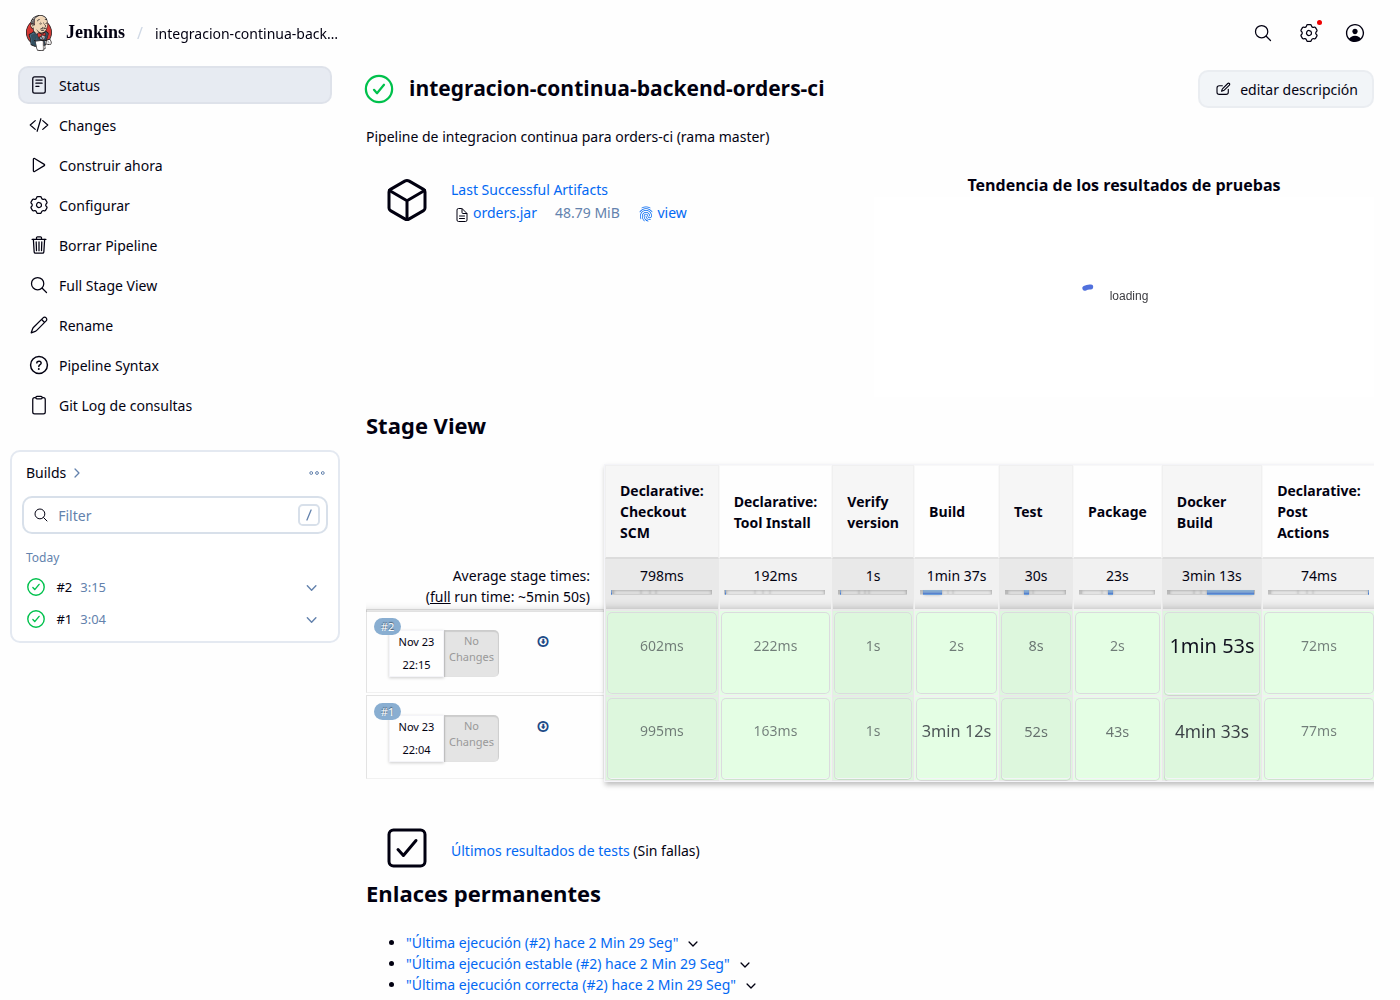
\includegraphics[width=0.92\textwidth]{evidencias_entrega2/capturas/01_job_stage_view.png}
\caption{Página del job con la vista de etapas (\texttt{pipeline-stage-view}) tras las ejecuciones
\#1 y \#2, con todas las etapas en verde y \texttt{orders.jar} como último artefacto.}
\label{fig:stageview}
\end{figure}

\begin{figure}[H]
\centering
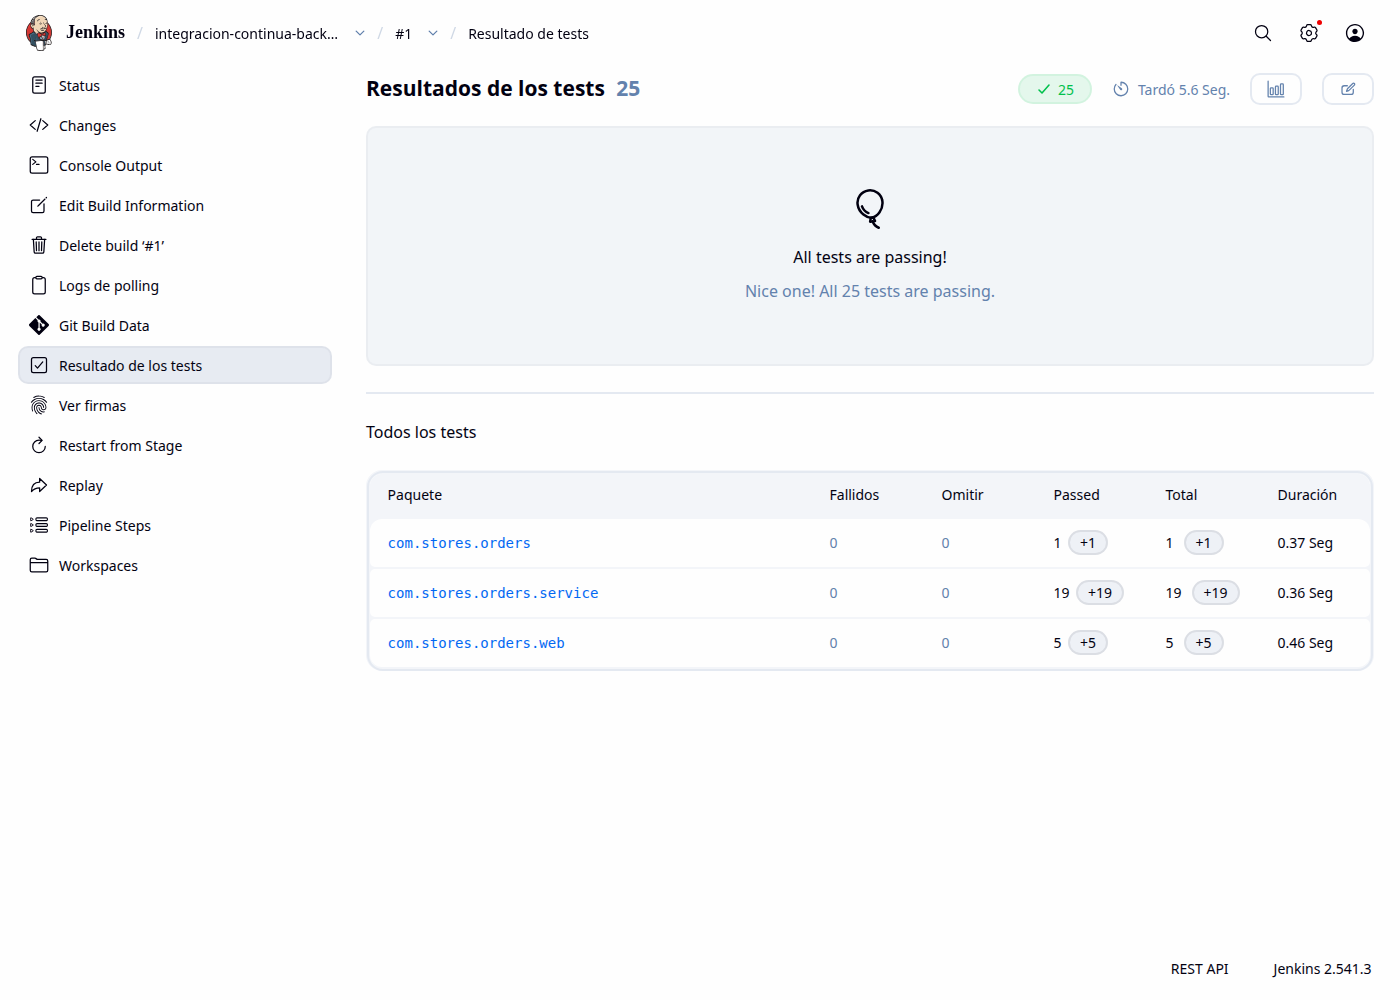
\includegraphics[width=0.92\textwidth]{evidencias_entrega2/capturas/03_build1_tests.png}
\caption{Reporte JUnit de la ejecución \#1 publicado por el paso \texttt{junit}: 25 pruebas aprobadas.}
\label{fig:testreport}
\end{figure}

\begin{figure}[H]
\centering
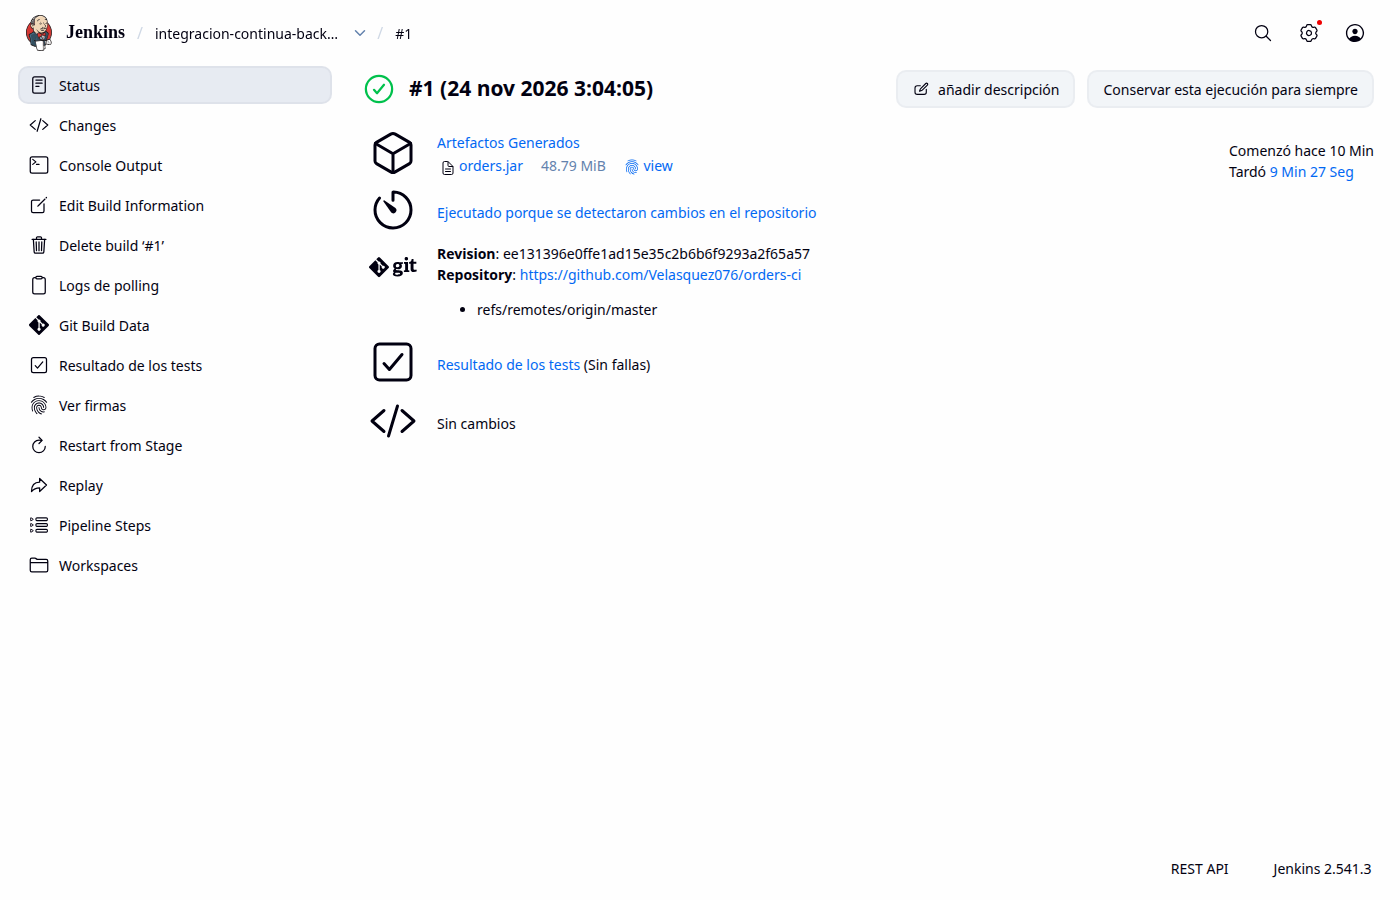
\includegraphics[width=0.49\textwidth]{evidencias_entrega2/capturas/02_build1_resumen.png}\hfill
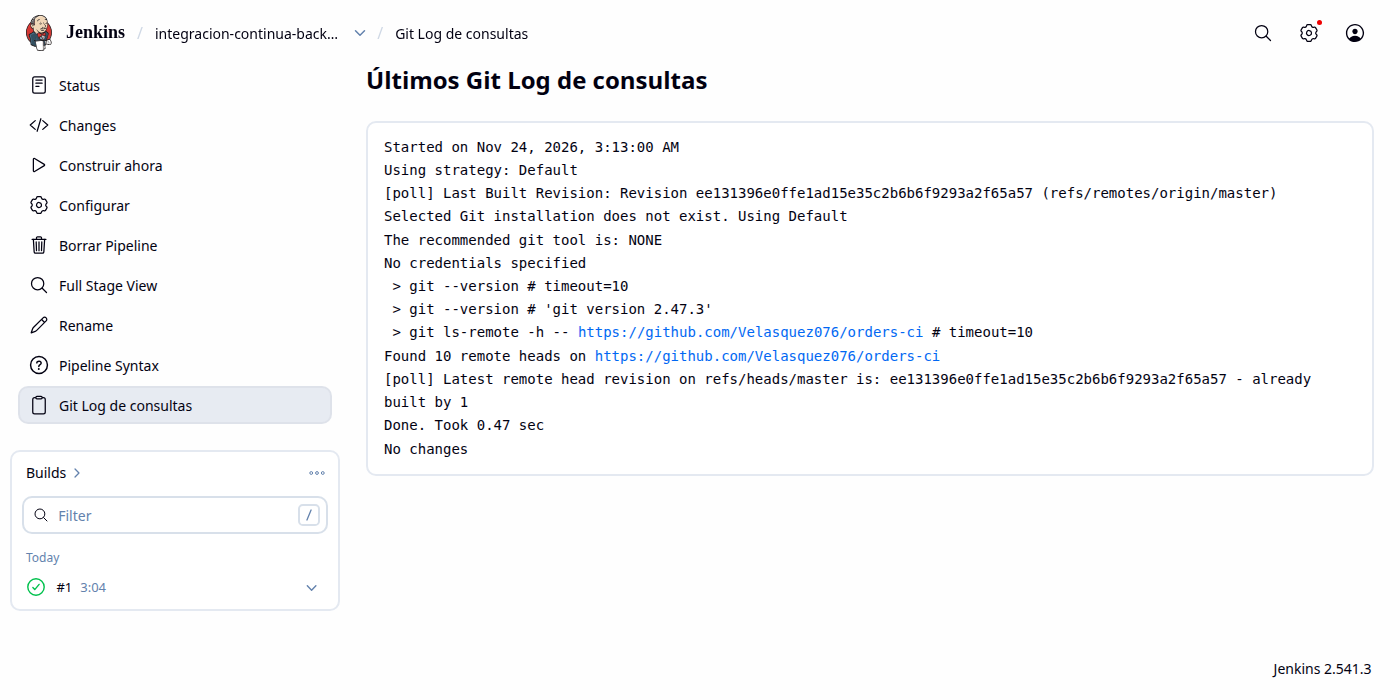
\includegraphics[width=0.49\textwidth]{evidencias_entrega2/capturas/05_polling_log.png}
\caption{Izquierda: resumen de la ejecución \#1, disparada por cambios en el repositorio, con revisión
\texttt{ee13139} y artefacto archivado. Derecha: registro de \emph{polling} del job.}
\label{fig:build1-polling}
\end{figure}

Estas ejecuciones confirman de forma directa la carga de JCasC, la creación del job con Job DSL, el
disparo por \emph{polling} y por \emph{webhook}, la resolución de herramientas, el acceso al socket, la
publicación JUnit, el archivado del artefacto y la construcción de la imagen. No reemplazan las
ejecuciones \#1--\#4 del servidor original, que siguen documentadas solo por el informe del equipo, y
no incluyen una ejecución con pruebas fallidas, porque provocarla exigiría introducir un error en el
código del backend.

\reservar{8cm}
\subsubsection*{Activación del \emph{webhook}}
\label{sec:webhook-real}
\addcontentsline{toc}{subsubsection}{Activación del \emph{webhook}}

Con permisos de administración sobre \texttt{Poligran-CI/orders-ci}, el 23 de noviembre de 2026 se
siguió el procedimiento de la sección~\ref{sec:webhook}, eligiendo \texttt{smee.io} como túnel
porque solo reenvía los eventos y no expone la interfaz de Jenkins a internet:
\begin{enumerate}[noitemsep]
  \item Se creó un canal en \texttt{smee.io} y se inició el cliente local \texttt{smee-client}, que
        reenvía cada evento a \texttt{http://localhost:8080/github-webhook/}.
  \item Se registró en el repositorio, con la API de GitHub, el \emph{webhook} \texttt{716049034}:
        destino el canal de \texttt{smee.io}, tipo \texttt{json}, solo el evento \emph{push},
        verificación SSL activa y sin secreto (\ruta{github_webhook_config.json}).
  \item Se arrancó Jenkins con \texttt{USE\_GITHUB\_WEBHOOK=true} y con \texttt{JENKINS\_BRANCH}
        apuntando a \texttt{feature/jenkins-portable}; Job DSL reemplazó \texttt{pollSCM} por
        \texttt{GitHubPushTrigger}.
\end{enumerate}

GitHub entregó tres eventos, todos con respuesta \texttt{200} (listado~\ref{lst:webhook-entregas}).
El \emph{ping} se recibió al crear el \emph{webhook}. El primer \emph{push}, al publicar la rama, se
recibió y \emph{tocó} el job, pero la consulta usó el SCM registrado en la ejecución \#2 (rama
\texttt{master}, ya construida) y terminó en \emph{No changes}
(\ruta{jenkins_webhook_push1_polling.txt}). Tras la ejecución manual \#3 con la nueva configuración,
el segundo \emph{push} (commit \texttt{b67c6a1}) encontró cambios y disparó la ejecución \#4
(listado~\ref{lst:webhook-poll}, figuras~\ref{fig:build4-webhook} y~\ref{fig:stageview-webhook}).

\begin{lstlisting}[caption={Entregas del \emph{webhook} según la API de GitHub y eventos registrados por Jenkins (UTC).},label={lst:webhook-entregas}]
2026-11-24T04:19:10Z  ping  200 OK
2026-11-24T04:19:23Z  push  200 OK
2026-11-24T04:24:00Z  push  200 OK
--- jenkins (docker logs) ---
04:19:11 PingGHEventSubscriber: PING webhook received from repo <https://github.com/Poligran-CI/orders-ci>!
04:19:23 DefaultPushGHEventSubscriber: Received PushEvent for https://github.com/Poligran-CI/orders-ci
04:19:23 Poked integracion-continua-backend-orders-ci
04:24:00 DefaultPushGHEventSubscriber: Received PushEvent for https://github.com/Poligran-CI/orders-ci
04:24:00 Poked integracion-continua-backend-orders-ci
\end{lstlisting}

\reservar{7cm}
\begin{lstlisting}[caption={\emph{GitHub Hook Log} del job tras el segundo \emph{push}: el evento provoca la consulta y esta encuentra cambios.},label={lst:webhook-poll}]
Started by event from 140.82.115.173:50206 => https://localhost:8080/github-webhook/
Using strategy: Default
[poll] Last Built Revision: Revision 5a76d6c39c818757eccd5b787b45fa429902426b (refs/remotes/origin/feature/jenkins-portable)
 > git ls-remote -h -- https://github.com/Poligran-CI/orders-ci # timeout=10
[poll] Latest remote head revision on refs/heads/feature/jenkins-portable is: b67c6a1a8f45d06c52f04b7466cf38b6f9eef255
Done. Took 0.46 sec
Changes found
\end{lstlisting}

\begin{figure}[H]
\centering
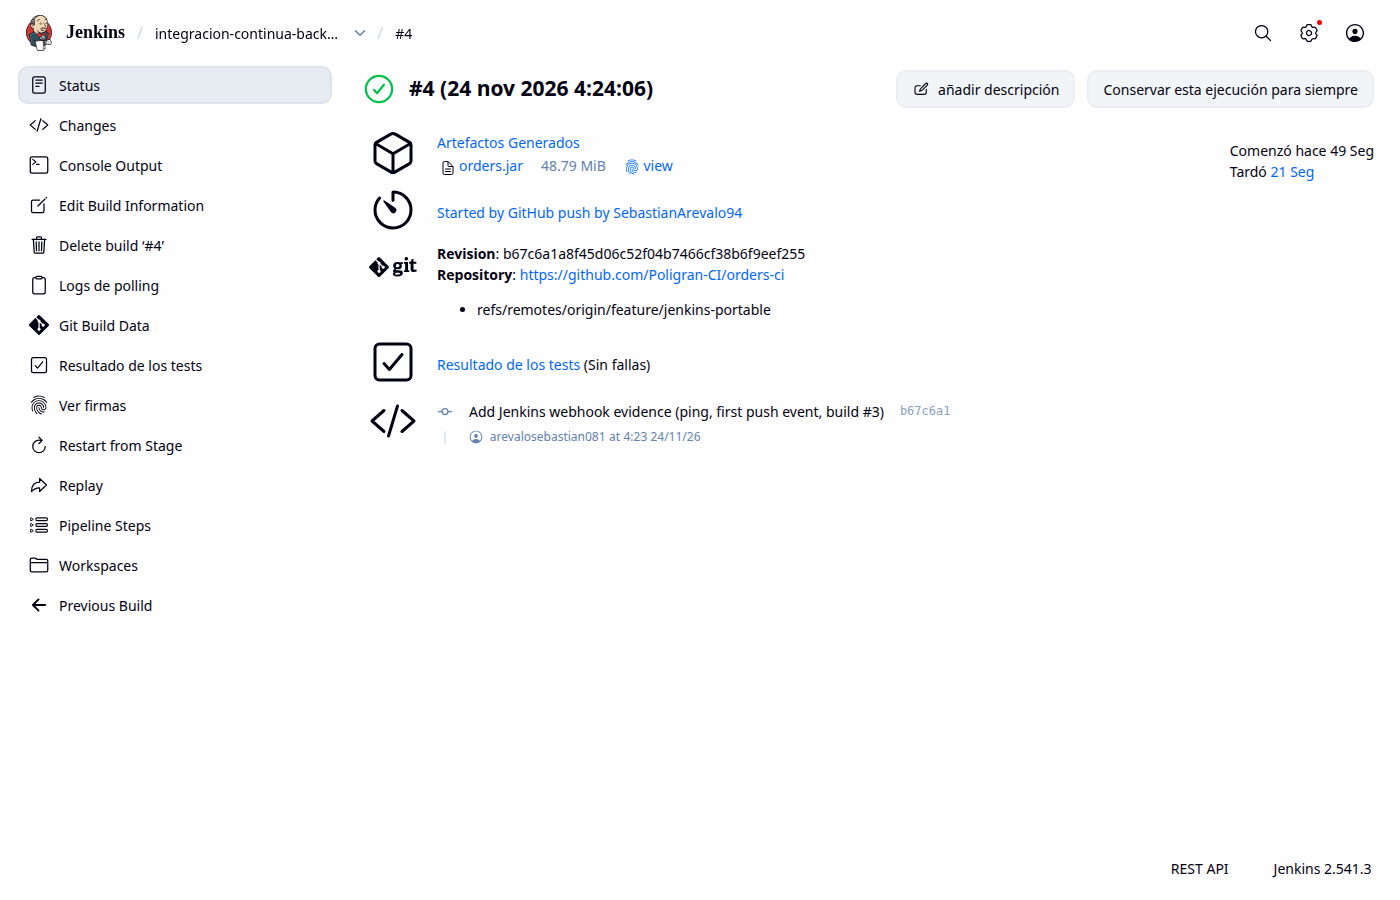
\includegraphics[width=0.86\textwidth]{evidencias_entrega2/capturas/06_build4_webhook.png}
\caption{Resumen de la ejecución \#4: causa \emph{Started by GitHub push by SebastianArevalo94},
revisión \texttt{b67c6a1} de \texttt{feature/jenkins-portable}, artefacto y pruebas sin fallos.}
\label{fig:build4-webhook}
\end{figure}

\begin{figure}[H]
\centering
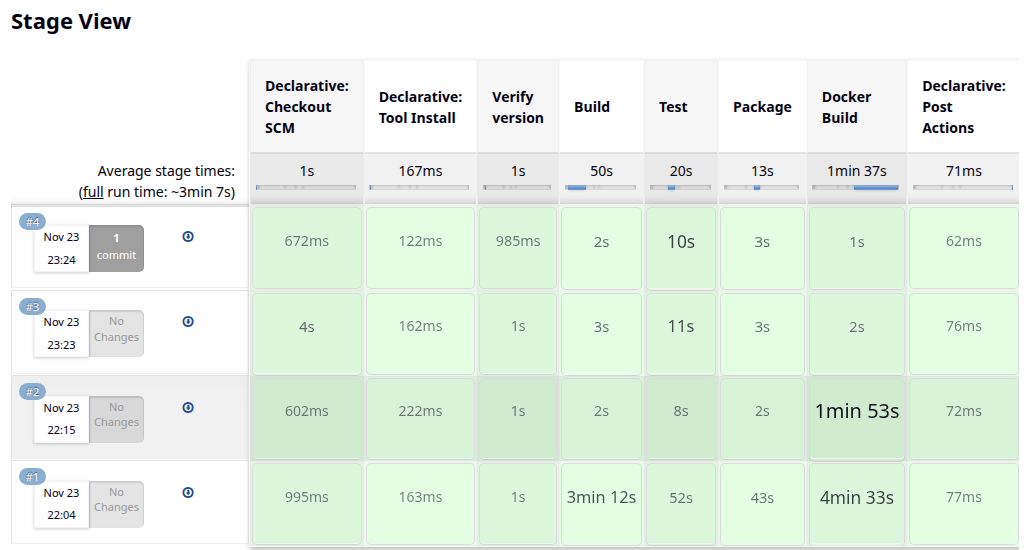
\includegraphics[width=0.80\textwidth]{evidencias_entrega2/capturas/08_job_stage_view_webhook.png}
\caption{Vista de etapas con las cuatro ejecuciones locales; la \#4 muestra el commit recibido por el
\emph{webhook}.}
\label{fig:stageview-webhook}
\end{figure}

El \emph{webhook} queda registrado en el repositorio, pero solo funciona mientras el cliente de
\texttt{smee.io} y Jenkins están en ejecución en este equipo; con ellos detenidos, las entregas
fallan sin afectar al repositorio. Para un uso permanente se necesita un Jenkins accesible de forma
estable y un secreto en el \emph{webhook}.

\reservar{16cm}
\subsection{Síntesis de evidencias}

\begin{table}[H]
\centering
\small
\begin{tabularx}{\textwidth}{@{}l P{4.1cm} L P{3.2cm}@{}}
\toprule
\textbf{Id} & \textbf{Evidencia} & \textbf{Qué demuestra} & \textbf{Requisito}\\
\midrule
E1 & \texttt{jenkins/Dockerfile}, \texttt{docker-compose.yml}, \texttt{plugins.txt} & Instalación
reproducible en contenedor con persistencia y plugins declarados. & Infraestructura, plugins\\
E2 & \texttt{jenkins/jenkins.yaml} & Seguridad, credencial, herramientas y job definidos como código. &
Configuración, credenciales, seguridad\\
E3 & \texttt{Jenkinsfile} & Pipeline declarativo del backend con pruebas, artefacto e imagen. &
Pipeline del backend\\
E4 & Ejecuciones \#1--\#3 (tabla~\ref{tab:builds}) & El pipeline se detiene y reporta la causa ante
fallos; correcciones versionadas. & Comportamiento ante errores\\
E5 & Ejecución \#4 (tabla~\ref{tab:builds}) & Ejecución completa en Jenkins: 25 pruebas, jar e
imágenes. & Pipeline, pruebas, imagen\\
E6 & Commits de la tabla~\ref{tab:commits} & Trazabilidad de la implementación y flujo de ramas. &
Historial de Git\\
E7 & Ejecuciones de Actions (tabla~\ref{tab:gha-runs}) & Validación de PR del backend y del frontend;
ausencia de ejecuciones por \emph{push} a \texttt{master}. & Relación con GitHub Actions; frontend\\
E8 & Listado~\ref{lst:verif-mvn} y anexo~\ref{anx:surefire} & Los comandos del pipeline funcionan
sobre el commit actual: 25/25 y \texttt{orders.jar}. & Pruebas y artefactos\\
E9 & Validación YAML y Compose & Los archivos de configuración son sintácticamente válidos. &
Configuración\\
E10 & Construcción de la imagen (sección~\ref{sec:verificacion}) & La etapa \emph{Docker Build}
funciona sobre el commit actual. & Imágenes Docker\\
E11 & Ejecución \#1 en Jenkins (tabla~\ref{tab:builds-local}, listado~\ref{lst:jenkins-console}) &
Pipeline completo en Jenkins, disparado por \emph{polling}, con 25 pruebas, jar e imagen. &
Pipeline, pruebas, artefactos, imagen, detección de cambios\\
E12 & \texttt{scm-polling.log} (listado~\ref{lst:polling}) & Funcionamiento del mecanismo de
consulta periódica. & Integración con GitHub\\
E13 & Capturas (figuras~\ref{fig:stageview}--\ref{fig:build1-polling}) & Vista de etapas, reporte
JUnit, resumen de ejecución y \emph{polling} en la interfaz de Jenkins. & Evidencias de ejecución\\
E14 & Ejecución \#2 y lista de plugins instalados & Disparo manual, caché, BuildKit;
plugins efectivamente instalados. & Plugins, imagen Docker\\
E15 & \emph{Webhook} \texttt{716049034}, entregas, registros y ejecución \#4
(listados~\ref{lst:webhook-entregas}--\ref{lst:webhook-poll}, figuras~\ref{fig:build4-webhook}
y~\ref{fig:stageview-webhook}) & Un \emph{push} a GitHub dispara el pipeline sin \emph{polling}. &
\emph{Webhooks}, detección de cambios\\
\bottomrule
\end{tabularx}
\caption{Evidencias, lo que demuestran y el requisito con el que se relacionan.}
\label{tab:evidencias}
\end{table}

\paragraph{Aspectos no verificables.} Duraciones, fechas exactas, registros y causas de disparo de las
ejecuciones \#1--\#4 del servidor original; recursos de hardware de ese servidor; número de
pruebas del frontend; una ejecución de Jenkins con pruebas fallidas.

\clearpage
% ===============================================================
\section{Estado de cumplimiento}
\label{sec:cumplimiento2}
% ===============================================================

\begin{longtable}{@{}P{3.4cm} P{4.6cm} P{3.6cm} P{2.7cm}@{}}
\toprule
\textbf{Requisito de la entrega} & \textbf{Implementación realizada} & \textbf{Evidencia disponible} &
\textbf{Estado}\\
\midrule
\endfirsthead
\toprule
\textbf{Requisito de la entrega} & \textbf{Implementación realizada} & \textbf{Evidencia disponible} &
\textbf{Estado}\\
\midrule
\endhead
Instalación de Jenkins & Contenedor Docker con imagen propia, Compose y volumen persistente &
E1, E9, E11 & \parcial{} (portable en una rama publicada, aún sin integrar en \texttt{master})\\
Configuración de Jenkins & JCasC + Job DSL; sin configuración manual & E2 & \ok\\
Plugins & 12 plugins declarados (80 instalados con dependencias); 9 en uso & E1, E14, tabla~\ref{tab:plugins} & \ok\\
Credenciales y secretos & \texttt{.env} no versionado; variables en JCasC; credencial cifrada &
E2, \texttt{.gitignore} & \parcial{} (token definido sin uso)\\
Seguridad & Usuario local, sin registro, sin acceso anónimo & E2, tabla~\ref{tab:seguridad} &
\parcial{} (sin roles; socket de Docker; \emph{webhook} sin secreto)\\
Pipeline del backend & \texttt{Jenkinsfile} declarativo de cinco etapas & E3, E5, E11 & \ok\\
Pruebas automatizadas en el pipeline & Etapa \emph{Test} + publicación JUnit & E5, E8, E11, E13 & \ok\\
Construcción de artefactos & \texttt{orders.jar} archivado con huella & E5, E8, E11 & \ok\\
Construcción de imágenes Docker & \texttt{orders-ci:<n>} y \texttt{latest} & E5, E10, E11, E14 &
\parcial{} (sin registro ni despliegue)\\
Comportamiento ante errores & Etapas que fallan detienen el pipeline; \texttt{post} & E4 & \ok\\
Pipeline del frontend en Jenkins & No implementado; solo GitHub Actions en rama sin integrar & E7 &
\pend\\
Detección de cambios en GitHub & \texttt{pollSCM H/2 * * * *} sobre \texttt{master}; \texttt{githubPush()} en modo \emph{webhook} & E2, E11, E12, E15 &
\ok\\
\emph{Webhooks} & \emph{Webhook} de \emph{push} activo vía \texttt{smee.io}; ejecución \#4 disparada por GitHub & E15 & \parcial{} (activo solo en la rama y con el equipo local encendido)\\
Evidencias de ejecución en Jenkins & Informe del equipo (\#1--\#4) y ejecuciones propias (\#1--\#4) & E4, E5, E11, E14, E15 &
\ok\\
Capturas y registros de consola de Jenkins & Capturas, consola, etapas y JUnit exportados & E11--E13, E15 & \ok\\
Arquitectura y diagramas & Figuras~\ref{fig:arquitectura} y~\ref{fig:flujo} & Este documento & \ok\\
Relación con GitHub Actions & Funciones complementarias; desajuste \texttt{main}/\texttt{master} &
E7, listado~\ref{lst:gha-trigger} & \parcial{}\\
Historial de commits & Commits de Jenkins trazables por rama & E6 & \ok\\
\bottomrule
\caption{Trazabilidad de los requisitos de la Entrega~2.}
\label{tab:cumplimiento2}
\end{longtable}

% ===============================================================
\section{Proyección hacia la tercera entrega}
\label{sec:proyeccion}
% ===============================================================

La implementación actual deja tres bases reutilizables: (1)~un \textbf{proceso de construcción
estandarizado} (\texttt{mvn clean compile}, \texttt{mvn test}, \texttt{mvn package},
\texttt{docker build}) que no depende de Jenkins y puede expresarse en cualquier servicio de
integración continua; (2)~una \textbf{batería de 25 pruebas} que funciona como criterio objetivo de
aceptación; y (3)~un \textbf{historial de ejecuciones} con el que comparar herramientas.

\paragraph{Evaluación de Travis CI y Codeship.} La tercera entrega contempla evaluar Travis CI y
Codeship, que \textbf{aún no se han implementado}. Ambos son servicios alojados que leen un archivo de
configuración del repositorio y se integran con GitHub mediante \emph{webhooks} gestionados por el
propio servicio \cite{travis-docs}, sin necesidad de túneles como el usado con la instalación
local. La comparación podrá hacerse con los mismos comandos y sobre el mismo commit,
usando como criterios: tiempo hasta la retroalimentación, esfuerzo de configuración, gestión de
secretos, soporte de Docker, publicación de reportes JUnit, costo y mantenimiento de
infraestructura (nulo en los servicios alojados, propio en Jenkins). La disponibilidad actual y las
condiciones de uso de ambos servicios deberán comprobarse en el momento de la evaluación.

\paragraph{Mejoras pendientes identificadas.}
\begin{itemize}[noitemsep]
  \item Pipeline de Jenkins para el frontend (Node.js~22: \texttt{npm ci}, \texttt{npm test},
        \texttt{npm run build}) tras integrar \texttt{feature/frontend}.
  \item Integrar la corrección del disparador de GitHub Actions (\texttt{0bad97e}).
  \item Añadir un secreto al \emph{webhook} y alojar Jenkins en un servidor accesible de forma
        estable, en lugar de depender de \texttt{smee.io} y de un equipo personal.
  \item Revisar e integrar en \texttt{master} la rama \texttt{feature/jenkins-portable}, que ya
        sustituye los montajes del anfitrión por herramientas dentro de la imagen y corrige la URL
        del repositorio para el \emph{webhook}.
  \item Publicar la imagen en un registro y desplegarla automáticamente en el ambiente \texttt{dev}
        con \texttt{docker compose}, avanzando hacia la entrega continua.
  \item Añadir \texttt{timeout}, limpieza del espacio de trabajo y de imágenes antiguas, y
        notificaciones del resultado.
  \item Mantener la exportación de capturas y registros de cada ejecución, como se hizo en la
        sección~\ref{sec:jenkins-local}, y documentar una ejecución con pruebas fallidas.
\end{itemize}

% ===============================================================
\section{Conclusiones}
\label{sec:conclusiones}
% ===============================================================

\subsection{Entrega 1: pruebas automatizadas}

\begin{itemize}
  \item La aplicación cubre el cálculo del total con descuentos y la validación de existencias contra
        una base de datos, con 25 pruebas automáticas que pasan y se ejecutan con un solo comando.
  \item La prueba \texttt{CP04} reproduce el error de doble descuento del caso y garantiza que no vuelva
        a producción.
  \item El comportamiento se definió primero en una especificación con entradas y resultados
        esperados; el historial de Git no refleja el orden pruebas-antes-que-código, y se documenta
        esa limitación en lugar de ocultarla.
  \item Frente a la revisión manual mensual, la automatización detecta los errores en minutos en vez
        de semanas, elimina un costo recurrente y ofrece una verificación completa y repetible.
\end{itemize}

\subsection{Entrega 2: integración continua con Jenkins}

\begin{itemize}
  \item Se implementó un servidor Jenkins en contenedor, configurado íntegramente como código (JCasC
        y Job DSL), que detecta cada cambio de \texttt{master} y ejecuta un pipeline declarativo de
        cinco etapas. Según el informe del equipo, la ejecución \#4 completó el pipeline con 25
        pruebas aprobadas, el \texttt{.jar} archivado y la imagen Docker construida. Con la misma
        configuración, una instalación propia obtuvo cuatro ejecuciones exitosas, la primera
        disparada por \emph{polling} y la cuarta por un \emph{webhook} de GitHub, con capturas,
        registros y reportes exportados.
  \item Las tres ejecuciones fallidas mostraron el valor del enfoque: cada problema se detectó en una
        etapa concreta, con un mensaje explícito, y se corrigió con un cambio versionado.
  \item Frente al proceso convencional, la ejecución de las pruebas deja de depender de una persona:
        ocurre siempre, con las mismas herramientas, y bloquea la generación de artefactos cuando
        falla una prueba.
  \item Las limitaciones son claras: en \texttt{master} la instalación depende de rutas de un equipo
        concreto (resuelto en \texttt{feature/jenkins-portable}, pendiente de integrar) y
        \texttt{DOCKER\_GID} solo se aplica con \texttt{--env-file}; el \emph{webhook} solo funciona
        en la rama y con el equipo local encendido, y no tiene secreto; todo usuario autenticado es
        administrador y el socket de Docker otorga
        control del anfitrión; no hay registro de imágenes ni despliegue; y el frontend no tiene
        pipeline en Jenkins.
\end{itemize}

\subsection{Relación con el diagnóstico y los indicadores de la Entrega 1}

El diagnóstico inicial identificó que el error de doble descuento podía permanecer hasta 30 días
porque el control era una revisión manual mensual. La tabla~\ref{tab:indicadores} retoma los aspectos
de la tabla~\ref{tab:manual-vs-auto} y muestra cómo cambia cada uno con Jenkins.

\begin{table}[H]
\centering
\small
\begin{tabularx}{\textwidth}{@{}P{2.6cm} L L L@{}}
\toprule
\textbf{Indicador} & \textbf{Revisión manual} & \textbf{Entrega 1 (pruebas)} & \textbf{Entrega 2 (Jenkins)}\\
\midrule
Momento de detección & Hasta 30 días & Cuando alguien ejecuta \texttt{mvn test} & En cada cambio de
\texttt{master}: hasta $\sim$2 min de \emph{polling} más la duración del pipeline\\
Dependencia de personas & Total & Ejecución manual & Ninguna para ejecutar; sí para corregir\\
Repetibilidad & Variable & Idéntica en cada ejecución & Idéntica, con herramientas fijadas por JCasC\\
Errores que vuelven & Pueden reaparecer & \texttt{CP04} falla & \texttt{CP04} falla y se bloquean
el \texttt{.jar} y la imagen\\
Evidencia & Informes manuales & Salidas guardadas a mano en \texttt{evidencias/} & Historial de
ejecuciones, reportes JUnit y artefactos en Jenkins\\
\bottomrule
\end{tabularx}
\caption{Evolución de los indicadores de la Entrega~1.}
\label{tab:indicadores}
\end{table}

En términos de la ecuación~\eqref{eq:perdida}, Jenkins reduce $d$ (días hasta la detección) al tiempo
de una ejecución del pipeline para todo cambio que llegue a \texttt{master}, sin depender de que una
persona recuerde ejecutar las pruebas. En la instalación propia, el pipeline completo tardó 9 min
27 s con la caché vacía y 2 min 14 s con la caché disponible; las pruebas ocuparon 52 s y 9 s,
respectivamente (tabla~\ref{tab:builds-local}). Así, $d$ pasa de hasta 30 días a unos pocos minutos.
La duración en el servidor original no se registró y deberá medirse con su propio historial.

% ===============================================================
\begin{thebibliography}{99}
% ===============================================================
\addcontentsline{toc}{section}{Referencias}

\bibitem{fowler-ci} M.~Fowler, ``Continuous Integration,'' \emph{martinfowler.com}, 2024.
  [En línea]. Disponible: \url{https://martinfowler.com/articles/continuousIntegration.html}

\bibitem{humble-farley} J.~Humble y D.~Farley, \emph{Continuous Delivery: Reliable Software Releases
  through Build, Test, and Deployment Automation}. Boston, MA, EE.\,UU.: Addison-Wesley, 2010.

\bibitem{jenkins-pipeline} Jenkins Project, ``Pipeline'' y ``Pipeline Syntax,'' \emph{Jenkins User
  Handbook}. [En línea]. Disponible: \url{https://www.jenkins.io/doc/book/pipeline/syntax/}

\bibitem{jenkins-docker} Jenkins Project, ``Installing Jenkins: Docker,'' \emph{Jenkins User
  Handbook}. [En línea]. Disponible: \url{https://www.jenkins.io/doc/book/installing/docker/}

\bibitem{jenkins-jcasc} Jenkins Project, ``Configuration as Code,'' \emph{Jenkins User Handbook}.
  [En línea]. Disponible: \url{https://www.jenkins.io/doc/book/managing/casc/}

\bibitem{jenkins-jobdsl} Jenkins Project, ``Job DSL Plugin.'' [En línea]. Disponible:
  \url{https://plugins.jenkins.io/job-dsl/}

\bibitem{jenkins-github} Jenkins Project, ``GitHub Plugin.'' [En línea]. Disponible:
  \url{https://plugins.jenkins.io/github/}

\bibitem{jenkins-security} Jenkins Project, ``Securing Jenkins'' y ``Controller Isolation,''
  \emph{Jenkins User Handbook}. [En línea]. Disponible:
  \url{https://www.jenkins.io/doc/book/security/controller-isolation/}

\bibitem{docker-socket} Docker Inc., ``Docker Engine security: Docker daemon attack surface.''
  [En línea]. Disponible: \url{https://docs.docker.com/engine/security/}

\bibitem{github-webhooks} GitHub, ``About webhooks,'' \emph{GitHub Docs}. [En línea]. Disponible:
  \url{https://docs.github.com/en/webhooks/about-webhooks}

\bibitem{github-actions} GitHub, ``Workflow syntax for GitHub Actions,'' \emph{GitHub Docs}.
  [En línea]. Disponible:
  \url{https://docs.github.com/en/actions/reference/workflows-and-actions/workflow-syntax}

\bibitem{travis-docs} Travis CI, ``Travis CI Documentation.'' [En línea]. Disponible:
  \url{https://docs.travis-ci.com/}

\end{thebibliography}

% ###############################################################
\clearpage
\appendix
\section{Anexo de evidencias}
\label{anx:evidencias}
% ###############################################################

\subsection{Entrega 1: pruebas en contenedor}

Extracto de \texttt{evidencias/05\_docker\_tests.txt} (8 de noviembre de 2026, Docker Desktop):

\begin{lstlisting}
=== 2026-11-08 12:05:33 -05 | sebastian@Sebastian-PC ===
Docker version 29.9.3, build 5457199
#0 building with "desktop-linux" instance using docker driver
...
[INFO] Tests run: 25, Failures: 0, Errors: 0, Skipped: 0
[INFO] BUILD SUCCESS
[INFO] Total time:  11.984 s
[INFO] Finished at: 2026-11-08T17:05:51Z
\end{lstlisting}

Las incidencias de la dockerización (API aislada sin base de datos y ruta relativa del script) y su
corrección se documentan en \texttt{docs/DOCKER\_INCIDENCIAS.md}.

\subsection{Entrega 2: mensajes de las ejecuciones fallidas de Jenkins}

Transcritos de \ruta{docs/JENKINS_CONFIGURACION.md}:

\begin{lstlisting}
# Build #1
Unable to find Jenkinsfile from git ...
# Build #2
Tool type "jdk" does not have an install of "JDK21" configured
Tool type "maven" does not have an install of "Maven3" configured
# Build #3
permission denied while trying to connect to the docker API at unix:///var/run/docker.sock
\end{lstlisting}

\subsection{Entrega 2: reportes JUnit de la verificación}
\label{anx:surefire}

\begin{table}[H]
\centering
\small
\begin{tabular}{@{}l r r r r r@{}}
\toprule
\textbf{Clase (\texttt{TEST-*.xml})} & \textbf{Pruebas} & \textbf{Fallos} & \textbf{Errores} &
\textbf{Omitidas} & \textbf{Tiempo (s)}\\
\midrule
\texttt{OrdersApplicationTests} & 1 & 0 & 0 & 0 & 3,788\\
\texttt{InventoryServiceTest} & 6 & 0 & 0 & 0 & 0,389\\
\texttt{OrderCalculatorTest} & 9 & 0 & 0 & 0 & 0,021\\
\texttt{OrderServiceTest} & 4 & 0 & 0 & 0 & 0,137\\
\texttt{OpenApiDocumentationTest} & 2 & 0 & 0 & 0 & 1,294\\
\texttt{OrderControllerTest} & 3 & 0 & 0 & 0 & 0,272\\
\midrule
\textbf{Total} & \textbf{25} & \textbf{0} & \textbf{0} & \textbf{0} & \\
\bottomrule
\end{tabular}
\caption{Resumen de \texttt{target/surefire-reports/} de la verificación del 23 de noviembre de 2026.}
\label{tab:surefire}
\end{table}

\subsection{Archivos de evidencia de la Entrega 2}

\begin{table}[H]
\centering
\small
\begin{tabularx}{\textwidth}{@{}l L@{}}
\toprule
\textbf{Archivo (\texttt{docs/entrega/evidencias\_entrega2/})} & \textbf{Contenido}\\
\midrule
\texttt{jenkinsfile\_stages\_local.txt} & Salida completa de las etapas Maven del
\texttt{Jenkinsfile} reproducidas sobre \texttt{ee13139}.\\
\texttt{docker\_build\_local.txt} & Salida de la etapa \emph{Docker Build} reproducida y metadatos de
la imagen.\\
\texttt{surefire\_resumen.txt} & Resumen por clase de los reportes JUnit generados.\\
\texttt{github\_actions\_runs.txt} & Ejecuciones y pasos de GitHub Actions consultados con \texttt{gh}.\\
\texttt{validaciones.txt} & Validación YAML y Compose, rama por defecto, disparador de Actions y
consulta de \emph{webhooks} previa a obtener permisos.\\
\texttt{jenkins\_local\_build.txt} & Construcción de la imagen de Jenkins, hallazgo de
\texttt{DOCKER\_GID}, herramientas del contenedor y carga de JCasC.\\
\texttt{jenkins\_build\{1..4\}\_console.txt} & Consola completa de las ejecuciones \#1 a \#4.\\
\texttt{jenkins\_build\{1..4\}\_stages.json} & Etapas y duraciones (\texttt{wfapi/describe}).\\
\texttt{jenkins\_build\{1..4\}\_tests.json} & Reporte JUnit publicado por Jenkins.\\
\texttt{jenkins\_build\{1..4\}\_info.json} & Causa, fecha y duración.\\
\texttt{github\_webhook\_config.json} & Configuración del \emph{webhook}, sin la URL del canal.\\
\texttt{github\_webhook\_entregas.txt} & Entregas del \emph{webhook} (\emph{ping} y \emph{push}) con su código de respuesta.\\
\texttt{jenkins\_webhook\_eventos.txt} & Eventos de GitHub registrados en el log de Jenkins.\\
\texttt{jenkins\_webhook\_push\{1,2\}\_polling.txt} & \emph{GitHub Hook Log} de cada \emph{push}.\\
\texttt{jenkins\_plugins\_instalados.txt} & Plugins instalados y su versión.\\
\texttt{jenkins\_polling\_e\_imagenes.txt} & \texttt{scm-polling.log} e imágenes \texttt{orders-ci}.\\
\texttt{capturas/*.png} & Capturas de la interfaz de Jenkins (figuras~\ref{fig:stageview}--\ref{fig:build1-polling},
\ref{fig:build4-webhook} y~\ref{fig:stageview-webhook}).\\
\bottomrule
\end{tabularx}
\caption{Archivos de evidencia generados para la Entrega~2.}
\label{tab:archivos-evid}
\end{table}

\section{Registro de uso de inteligencia artificial}
\label{anx:ia}

\begin{table}[H]
\centering
\small
\begin{tabularx}{\textwidth}{@{}P{3.2cm} L@{}}
\toprule
\textbf{Aspecto} & \textbf{Detalle}\\
\midrule
Herramienta & Claude Code (Anthropic), modelo Claude Opus 5.5.\\
Fecha & 23 de noviembre de 2026.\\
Uso & Análisis del repositorio (archivos, historial de Git, ramas y ejecuciones de GitHub Actions);
verificaciones en contenedores sobre una copia del commit \texttt{ee13139}; a petición del equipo,
creación de la rama \texttt{feature/jenkins-portable}, ejecución de Jenkins, registro del
\emph{webhook} y exportación de evidencias; redacción de la Parte~II, diagramas e integración de ambas entregas en este documento.\\
Restricciones aplicadas & No se modificó el código de la aplicación ni el frontend; los cambios de
configuración de Jenkins se confirmaron y publicaron, a petición del equipo, solo en
\texttt{feature/jenkins-portable} (\texttt{master} no se modificó); no se incluyeron secretos. Los datos de las ejecuciones \#1--\#4 provienen del
informe del equipo y se identifican como tales.\\
Responsabilidad & El equipo revisa, valida y asume el contenido entregado.\\
\bottomrule
\end{tabularx}
\caption{Registro de uso de inteligencia artificial.}
\label{tab:ia}
\end{table}

\end{document}
